\documentclass[9pt,twocolumn,twoside,lineno]{pnas-new}

%% Some pieces required from the pandoc template
\providecommand{\tightlist}{%
  \setlength{\itemsep}{0pt}\setlength{\parskip}{0pt}}

% Use the lineno option to display guide line numbers if required.
% Note that the use of elements such as single-column equations
% may affect the guide line number alignment.


\usepackage[T1]{fontenc}
\usepackage[utf8]{inputenc}


\usepackage{eso-pic,graphicx,transparent,xcolor}

\templatetype{pnasresearcharticle}  % Choose template

\title{The Regional Effects of Marine Protected Areas}

\author[a,1]{Daniel Ovando}
\author[b]{Jennifer E. Caselle}
\author[b]{Christopher Costello}
\author[b]{Olivier Deschenes}
\author[b]{Steven D. Gaines}
\author[a]{Ray Hilborn}
\author[b]{Owen Liu}

  \affil[a]{University of Washington, School of Aquatic and Fishery Sciences}
  \affil[b]{University of California, Santa Barbara}


% Please give the surname of the lead author for the running footer
\leadauthor{Ovando}

% Please add here a significance statement to explain the relevance of your work
\significancestatement{Healthy marine ecosystems are critical to the well-being of the planet.
Marine protected areas, parts of the oceans protected from human
activities such as fishing, are increasingly being used in an effort to
conserve and manage these ecosystems. Our study pairs theory with
empirical methods to examine the regional effects of MPAs on
conservation outcomes. Using simulations, we show that the regional
effects of marine protected areas can be highly variable and dependent
on human drivers. We find no statistically clear effect of a network of
MPAs after 13 years of protection, which our simulation analysis
suggests is actually to be expected. Our results lay a foundation for
future research on the design and monitoring of marine protected areas.}


\authorcontributions{D.O., S.G., and R.H. developed structure of simulation model. D.O.,
O.D., C.C., and J.C. developed estimation strategy. J.C. provided
support on collecting and interpreting data. All simulations,
statistics, and sensitivity analyses performed by D.O. and O.L. . All
authors contributed to the manuscript.}

\authordeclaration{R.H's research program receives funding from environmental NGOs,
foundations, fishing industry, governments and international agencies.
All of these can be interpreted as a conflict of interest when
evaluating fisheries policy. C.C., S.G., and O.D's research program
includes funding from environmental NGOs and foundations with an
interest in ocean conservation and food security. Funding for D.O. was
partly provided by the NMFS-Sea Grant Population and Ecosystem Dynamics
Fellowship.}


\correspondingauthor{\textsuperscript{} }

% Keywords are not mandatory, but authors are strongly encouraged to provide them. If provided, please include two to five keywords, separated by the pipe symbol, e.g:
 \keywords{  Marine Protected Areas |  Conservation |  Bio-economic modeling |  Program Evaluation  } 

\begin{abstract}
Marine Protected Areas (MPAs) cover between 3-7\% of the world's oceans,
up from less than 1\% in the year 2000. The Convention on Biological
Diversity calls for 10\% of coastal waters to be protected inside MPAs
by 2020, while the International Union for Conservation of Nature calls
for 30\% protection by 2030. It is often clear that MPAs produce
conservation benefits inside their borders, but many MPAs are also
justified on the grounds that they also benefit the broader region
outside their borders. The conservation effects of MPAs are most
commonly evaluated using response ratios---measures of biomass densities
inside their borders, relative to biomass densities in reference sites
outside their borders. Studies of this nature have provided broad
evidence that MPAs produce conservation benefits within their borders.
While these gains can be vitally important, marine populations are
rarely contained entirely within the borders of MPAs; therefore a
critical question is not only do MPAs produce conservation gains inside
their borders, but how do they affect the broader region in which they
are located? The Channel Islands National Marine Sanctuary provides a
clear example of this challenge. A network of MPAs covering roughly 20\%
of the Islands' waters was put in place in 2003, with a goal of
providing regional conservation and fishery benefits. Response ratios
from the region indicate that the Channel Island MPAs have increased
biomass densities inside the MPAs. However, we are unable to find a
clear effect of these same MPAs at the regional scale across multiple
species.Building off of existing theory, we use a bio-economic
simulation model to explain this discrepancy, and demonstrate under what
conditions we likely can and cannot clearly estimate the regional
conservation effects of MPAs. We show that MPA networks covering 25\% or
less of a region are likely to produce regional increases in fish
biomass on the order of 10\%-20\%, a meaningful effect but also one that
can easily be overwhelmed by environmental shocks. Our results provide a
novel assessment of the regional effects of a large and iconic Marine
Protected Area network, and provide guidance for managers charged with
monitoring and adapting MPAs.
\end{abstract}

\dates{This manuscript was compiled on \today}
\doi{\url{www.pnas.org/cgi/doi/10.1073/pnas.XXXXXXXXXX}}

\begin{document}

% Optional adjustment to line up main text (after abstract) of first page with line numbers, when using both lineno and twocolumn options.
% You should only change this length when you've finalised the article contents.
\verticaladjustment{-2pt}

\maketitle
\thispagestyle{firststyle}
\ifthenelse{\boolean{shortarticle}}{\ifthenelse{\boolean{singlecolumn}}{\abscontentformatted}{\abscontent}}{}

% If your first paragraph (i.e. with the \dropcap) contains a list environment (quote, quotation, theorem, definition, enumerate, itemize...), the line after the list may have some extra indentation. If this is the case, add \parshape=0 to the end of the list environment.

\acknow{Funding for the simulation model was provided by the NMFS-Sea Grant
Population and Ecosystem Dynamics Fellowship. This study would not be
possible without the work provided by PISCO divers over the years. DO
thanks Cody Szuwalski, Julia Lawson, and André Punt for helpful comments
and technical support.}

\emph{as we move away from ``set it and forget it'' management towards
adaptive management of marine ecosystems, it is critically important
that we develop robust strategies for monitoring the effectiveness of
our management intercentions}

No-take Marine Protected Areas (MPAs), spatial regions of the ocean in
which fishing is prohibited, have a long history in the management of
marine resources. Traditional cultures in Oceania utilized - often
temporary - MPAs as ``fish banks'' for times of need (1). Modern MPAs
were first established primarily as marine analogs to the terrestrial
protection of iconic landscapes like Yellowstone or Kruger National
Parks (2, 3). Over time our goals and expectations for MPAs have
evolved; while all MPAs are expected to deliver conservation benefits
within their borders, many modern MPAs are also established to bolster
fish populations throughout the region in which they are located (4).

Indeed, many recent agreements to expand MPAs (most proximately, the
Convention on Biological Diversity's Strategic Plan for Biodiversity,
which calls for 10\% of coastal waters to be protected inside MPAs by
2020 and the International Union for Conservation of Nature call for
30\% by 2030) are based on the expectaion that well-designed MPAs will
achieve benefits both within, and outside, their borders. Despite these
assumptions, our collective scientific understanding of the
regional-scale conservation and fishery impacts of current and future
MPAs is surprisingly limited.

Numerous studies provide evidence that well-enforced and appropriately
sized MPAs can produce conservation benefits within their borders
(5--8). As these conservation benefits accrue inside MPAs, theory holds
that MPAs can affect the waters beyond their borders through the
spillover of adult and larval fish from the protected to the fished
areas, as well as through displacement of fishing effort. Several
studies have documented empirical evidence for the existence of adult or
larval spillover affecting both abundance and fisheries (9--17), as well
as alteration of fishing effort in reaction to (18--20) and in
anticipation of (21) MPA placement. The potentially more important
question, however, is not whether spillover occurs (it must to some
degree in any realistic scenario), but what the net effects of spillover
are and whether those effects are empirically detectable. From a fishery
perspective, are spillover benefits sufficient to offset losses in
fishing grounds and changes in responses of displaced fishers caused by
an MPA? From a conservation perspective, how much does the buildup of
fish inside an MPA increase biomass outside the protected area? Overall,
what are the regional effects of MPAs?

As stakeholders around the world increasingly seek to use MPAs in marine
resource management portfolios, it is critical that we develop a better
understanding of the magnitude and drivers of regional-scale MPA
effects. This is particuarly true in the context of a changing climate,
in which ``set it and forget it'' management strategies are increasinly
untenable; we need to be able to monitor the performance of MPAs in
order to adapt them as dictated by a shifting environment. The Channel
Islands National Marine Sanctuary, California, USA provides an ideal
case study to address this need. A network of protected areas covering
approximately 20\% of the Islands' waters was put in place in 2003 (22).
This MPA network has subsequently been used as a model case study in
protected area design around the world XX.

We use data from the first 14 years of protection to provide what is to
our knowledge the first empirical assessment of the regional effect of a
large MPA network on a wide array of finfish species. In contrast to
clear differences in biomass densities observed inside and outside of
well protected MPAs both globally (5) and in the Channel Islands
({\textbf{???}}) we are unable to detect a clear regional effect from
the Channel Islands MPAs. We build off of existing MPA theory to
consider why this might be, and provide guidance for scientists and
managers as to when and how we might expect to estimate the regional
conservation effects of MPAs.

\hypertarget{what-are-the-regional-effects-of-mpas}{%
\subsection*{What Are the Regional Effects of
MPAs?}\label{what-are-the-regional-effects-of-mpas}}
\addcontentsline{toc}{subsection}{What Are the Regional Effects of
MPAs?}

The empirical MPA literature has generally focused on assessing
conservation effects within the borders of protected areas (7). While
these within-MPA effects are vitally important for protecting rare
species, biodiversity, critical habitats, and often tourism, they paint
an incomplete picture of the overall population effects of MPAs. The
organisms within the borders of protected areas are generally part of a
broader biological stock, connected through adult movement and larval
dispersal. If the goal of conservationists or natural resource managers
is to increase the total abundance or productivity of a resource, a
broader question we should ask of MPAs is not just are there more fish
inside their borders, but also how have reserves affected populations
throughout the region in which they are located? This logic, that MPAs
will have conservation benefits for most species beyond their borders,
is implicit in all multilateral calls for MPA expansion.

We define the regional conservation effects of MPAs as the change in
total biomass densities of fish (averaging inside and outside of MPAs)
relative to the total biomass densities of fish that would have occurred
without the MPAs (acknowledging that other outcomes such as increased
biodiversity or resiliency are also important to conservation but are
beyond the scope of this analysis). Numerous factors can affect the
regional effects of MPAs. These include the scale of adult and larval
dispersal relative to the size of the MPAs (8, 26--29), larval dispersal
patterns and the strength and timing of density dependence in the
population (e.g.~pre- or post-settlement, \textbf{???}), how overfished
the population would be without the MPA, and how fishing and management
responds to the implementation of the MPAs ({\textbf{???}}, 4, 30--39).
In addition, even for the same total area of MPAs, the location and
spacing of the MPAs can have a profound influence on their cumulative
impact through habitat and network effects (4, 40).

Given this existing body of theory, what should we expect \emph{a
priori} the effect size of the Channel Islands MPAs to be? While we know
many parameters will affect the expected effects of the MPAs, theory
suggests that life history, adult and larval dispersal relative to MPA
size, and fishing pressure will be key drivers. The targeted species in
our database span a range of life histories, but are largely made up of
fishes in the genus XX (e.g.) and \textbf{Sebastes} (e.g.~), with a
median Von Bertalanffy growth coefficient of XX, and a median age at
maturity of XX (41). The MPAs in this study cover 21\% of the the
surface waters of the Northern Channel Islands, a region spanning
roughly 90km east to west. While detailed dispersal studies are not
available for all of the species covered by our study, what information
we have suggest that while adults of some of these species are likely to
exhibit some site fidelity (42), larvae are likely distributed beyond
the northern Channel Islands (43). Therefore, if we assume that the
population of the targeted species is at least equal to the extent of
the Northern Channel Islands, we can assume that at most the MPAs cover
roughly 20\% of the targeted populations' ranges.

Turning to the critical question of fishing pressure, formal stock
assessments are largely lacking for these species. However, what
evidence we have suggests mostly moderate fishing pressure, with some
species such as California sheephead (\emph{Semicossyphus pulcher}) and
blue rockfish (\emph{Sebastes mystinus}) experiencing high levels of
fishing mortality / biomass levels below target levels during the early
2000s (44, 45). We integrated these network design features, life
history traits, and exploitation histories into a spatially explicit
bio-economic simulation model, and used this model to generate expected
outcomes for the Channel Islands MPAs. Our results suggest that while a
wide range of outcomes are plausible, from 0\% to upwards of 200\%,
across the majority of our simulations the effect size was 25\% or less,
with a median simulated effect size of roughly 20\%; a potentially small
value given the natural variability and sampling challenges of marine
environments.

\hypertarget{how-can-we-detect-regional-effects}{%
\subsection{How Can We Detect Regional
Effects?}\label{how-can-we-detect-regional-effects}}

Having established a theoretical grounding for the likely biomass
density outcomes of the Channel Island MPAs, what empirical evidence do
we have of the effects? \textbf{???} examined changes in biomass
densities of species targeted by fishing activity inside and outside of
the MPAs over time (a metric generally termed a ``response ratio''), and
compared these changes to the trends in non-targeted species. They found
a statistically significant increase in the response ratios of targeted
species over time, and evidence that this increase is smaller in the
non-targeted species. Updating the results of (46) through 2017 with a
Bayesian response-ratio regression shows a continuation of the
increasing trend in the response ratios of targeted species
(Fig.@ref(fig:XX)).

Why do these response ratio results not serve as sufficient evidence for
the regional effects of the Channel Island MPAs? Control sites used in
calculating response ratios are often selected based on abiotic or
ecological traits such as habitat characteristics (47). However,
selection of control sites is further complicated by the very spillover
that MPAs are often intended to create. Export of adults or larvae from
the MPA to the ``control'' site affects their status as controls, as
does displacement of fishing effort from MPAs to control sites. In
theory, control sites far enough away to negate both biological
spillover and concentration by the fishing fleet could be selected, but
finding suitably far sites that are also appropriate proxies for the
ecological and economic context of the MPAs may be challenging. While
these concerns have been stated previously (48), the MPA evaluation
literature has by and large been unable to adequately address them,
often due to the very real logistical challenges of identifying and
sampling adequate control sites that are truly independent of the MPAs
in question. As a result of these challenges, response ratios can be a
highly imprecise and biased measure of the regional conservation effect
of an MPA network (47).

In the case of the Channel Islands MPAs, control sites are often located
within only a few kilometers of an MPA, suggesting that they are
susceptible to biological spillover and concentration of fishing effort
resulting from the MPAs. Given these complications, we can certainly
interpret the response ratios reported in (46) and updated here as
evidence that the MPAs are providing effective protection of targeted
fish biomass inside their borders, particularly in light of the general
increase in response ratios over time. However, it is unclear how well
these response ratio results serve as in indicator of overall regional
effects of the MPAs.

To illustrate this problem, we used a bio-economic model to simulate
response ratio trajectories for species and MPA coverage representative
of the northern Channel Islands (see methods and SI for details of model
structure). These simulations cover the life-histories and MPA sizes
seen in the Channel Islands, but vary in key unknowns such as the actual
degree of fishing pressure, the timing of density dependence, and the
fleet responses to the MPAs. For each year of protection, we paired our
simulated response ratios to the estimated posterior probability
distributions of the Channel Island response ratios. For example, if the
mean estimated response ratio in the year 2006 is one, we found all
simulations with three years of protection that had simulated response
ratios near one, and then pulled out the ``true'' simulated regional MPA
effect from each of those simulations. This provides us with a
distribution of simulated regional MPA effects that could plausibly
generate the types of response ratios actually observed in the Channel
Islands.

As reported in (46), we see evidence for an increasing trend in response
ratios of targeted species over time (Fig.@ref(fig:rr-plot)). This
provides strong evidence that the MPAs are providing protection for
targeted species within their borders. However, our simulation results
show that the response ratio trends we observe in the data could
plausibly be produced by a wide range of regional MPA effects
(Fig.@ref(fig:rr-plot)). Response ratios well over one were associated
with regional MPA effects generally less than 25\%, and many simulations
produced large response ratios but regional MPA effects close to 0\%
This can occur if for example fishing pressure is only moderate, adult
movement is low, larval dispersal is high, and displaced fishing effort
concentrates around the border of the MPAs.

\textbackslash begin\{figure\emph{\}\%{[}tbhp{]} \centering
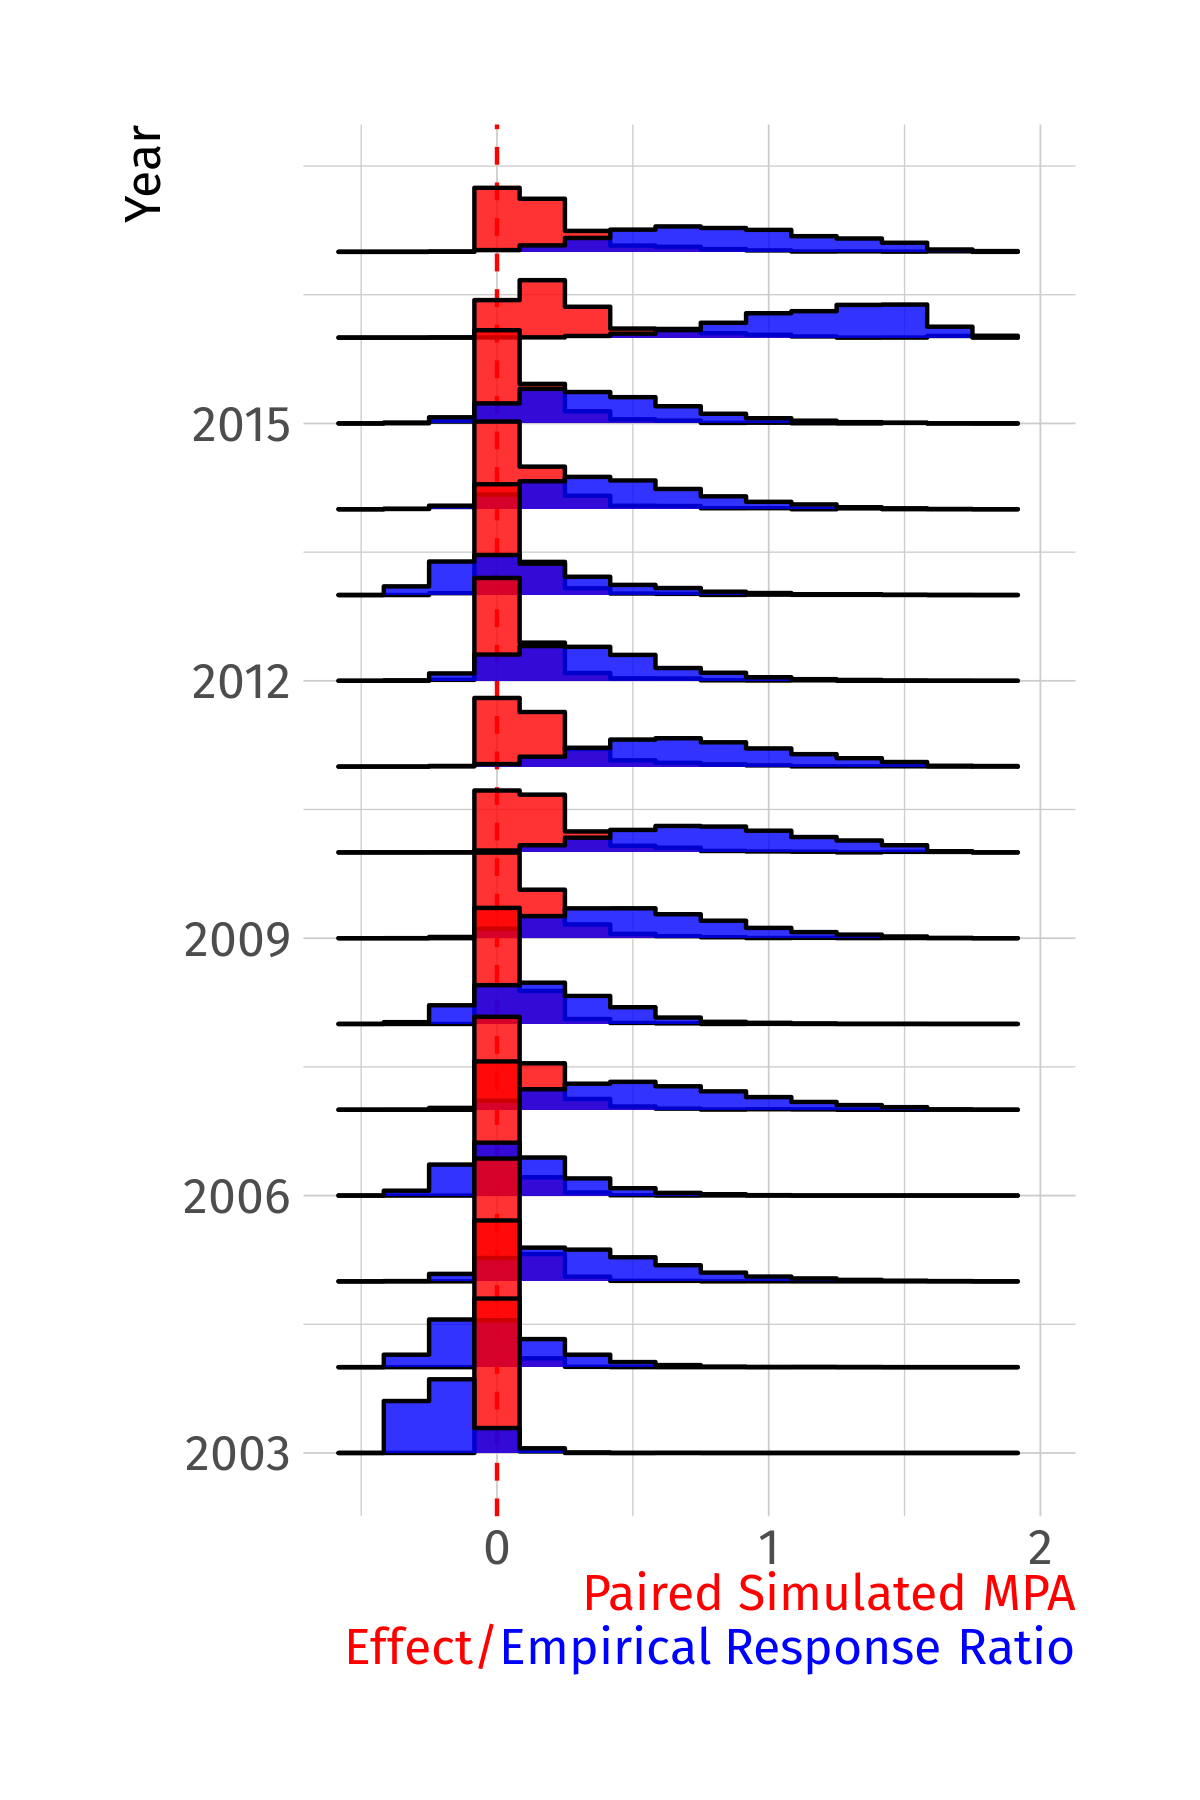
\includegraphics[width=.9\linewidth]{figs/response_ratio_plot.png}
\textbackslash caption\{90\% Posterior probability distributions of
response ratios for targeted species (x-axis) over time (y-axis) in
blue. Simulated MPA effects associated with simulated response ratios
matched to empirical response ratios in red. For response ratios, a
value of zero indicates that biomass densities of targeted and
non-targeted species are identical inside and outside MPAs, a value of 1
indicates that biomass densities of targeted species are 100\% greater
inside MPAs than outside. For MPA effect, a value of zero indicates that
mean biomass densities are identical in the with- and without- MPA
scenarios. A value of 1 indicates that mean biomass densities are 100\%
greater in the scenario with MPAs than the scenario without MPAs.\}
\label{rr-plot} \textbackslash end\{figure}\}

Given the potential unreliability of response ratios for the task, in an
ideal world how would we empirically measure the regional effects of
MPAs? The perfect experiment would involve two parallel worlds that were
identical, except for the implementation of an MPA. In world ``A'', no
MPA would be implemented, and in the facsimile world ``B'', the MPA
would be implemented. Both worlds would be tracked before and after MPA
implementation, and the biomass densities would be compared after
treatment. Instead of two parallel worlds, a similar experimental design
would involve random placement of MPAs. Unfortunately, neither of these
experimental designs has been implemented, because parallel worlds do
not exist and MPAs are to our knowledge never placed at random. Careful
causal inference requires some other means of controlling for biases
introduced by factors such as the unobserved environmental shocks, the
MPA siting process, biological spillover, and concentration of fishing
effort (47, 49).

Building off of the concepts explored in (46), we propose an alternative
identification strategy utilizing biomass densities of XX species that
are not directly targeted by fishing as our control group
(non-targeted), and biomass densities of XX species targeted by fishing
as our treatment group. Targeted species in the Northern Channel
Islands, California, include commercially important fin-fish such as
California sheephead (\emph{Semicossyphus pulcher}), and copper
(\emph{Sebastes caurinus}) and blue (\emph{Sebastes mystinus}) rockfish.
Each of these targeted species was the subject of prior bio-economic
modeling related to the effects of MPAs in southern California (50, 51).
It should be noted though that our analysis omits species from important
invertebrate fisheries including red urchin (\emph{Mesocentrotus
franciscanus}) and spiny lobster (\emph{Panulirus interruptus}).
Included non-targeted species include garibaldi (\emph{Hypsypops
rubicundus}), halfmoons (\emph{Medialuna californiensis}), and
blacksmith (\emph{Chromis punctipinnis}) (See Table.S2 for a complete
list of species). We used a Bayesian difference-in-difference regression
to estimate any difference in mean total biomass densities of fin-fish
species targeted by fishing effort (i.e., those potentially affected by
an MPA) and those species not targeted by fishing before and after MPA
implementation (49). The result of this regression is, conditional on
the assumptions of the model, an estimate of the effect of the MPAs on
the mean total biomass densities of targeted species throughout the
Channel Islands.

As conventional wisdom and theory would suggest, over the first three
years of implementation (2003-2006), the effects of the MPAs are
unclear, with support for a small negative effect to a substantially
positive effect (with much higher probability of a small positive
effect). Over the next six years the model estimates greater
probabilities of an increasingly positive MPA effect, peaking in
2009-2011 with a median estimate of MPA effect of a xx increase in mean
total biomass of targeted species (90\% credible interval 37\% - 128\%.
These empirical estimates are in line with (though in the upper range
of) the outcomes that our simulation model suggests are plausible given
the rough characteristics of the northern Channel Island MPAs. However,
in the subsequent years the trend reverses itself, and for the years
2015-2017 we once again see no clear effect of the MPAs
Fig.@ref(fig:mpa-effect)

\textbackslash begin\{figure\emph{\}\%{[}tbhp{]} \centering
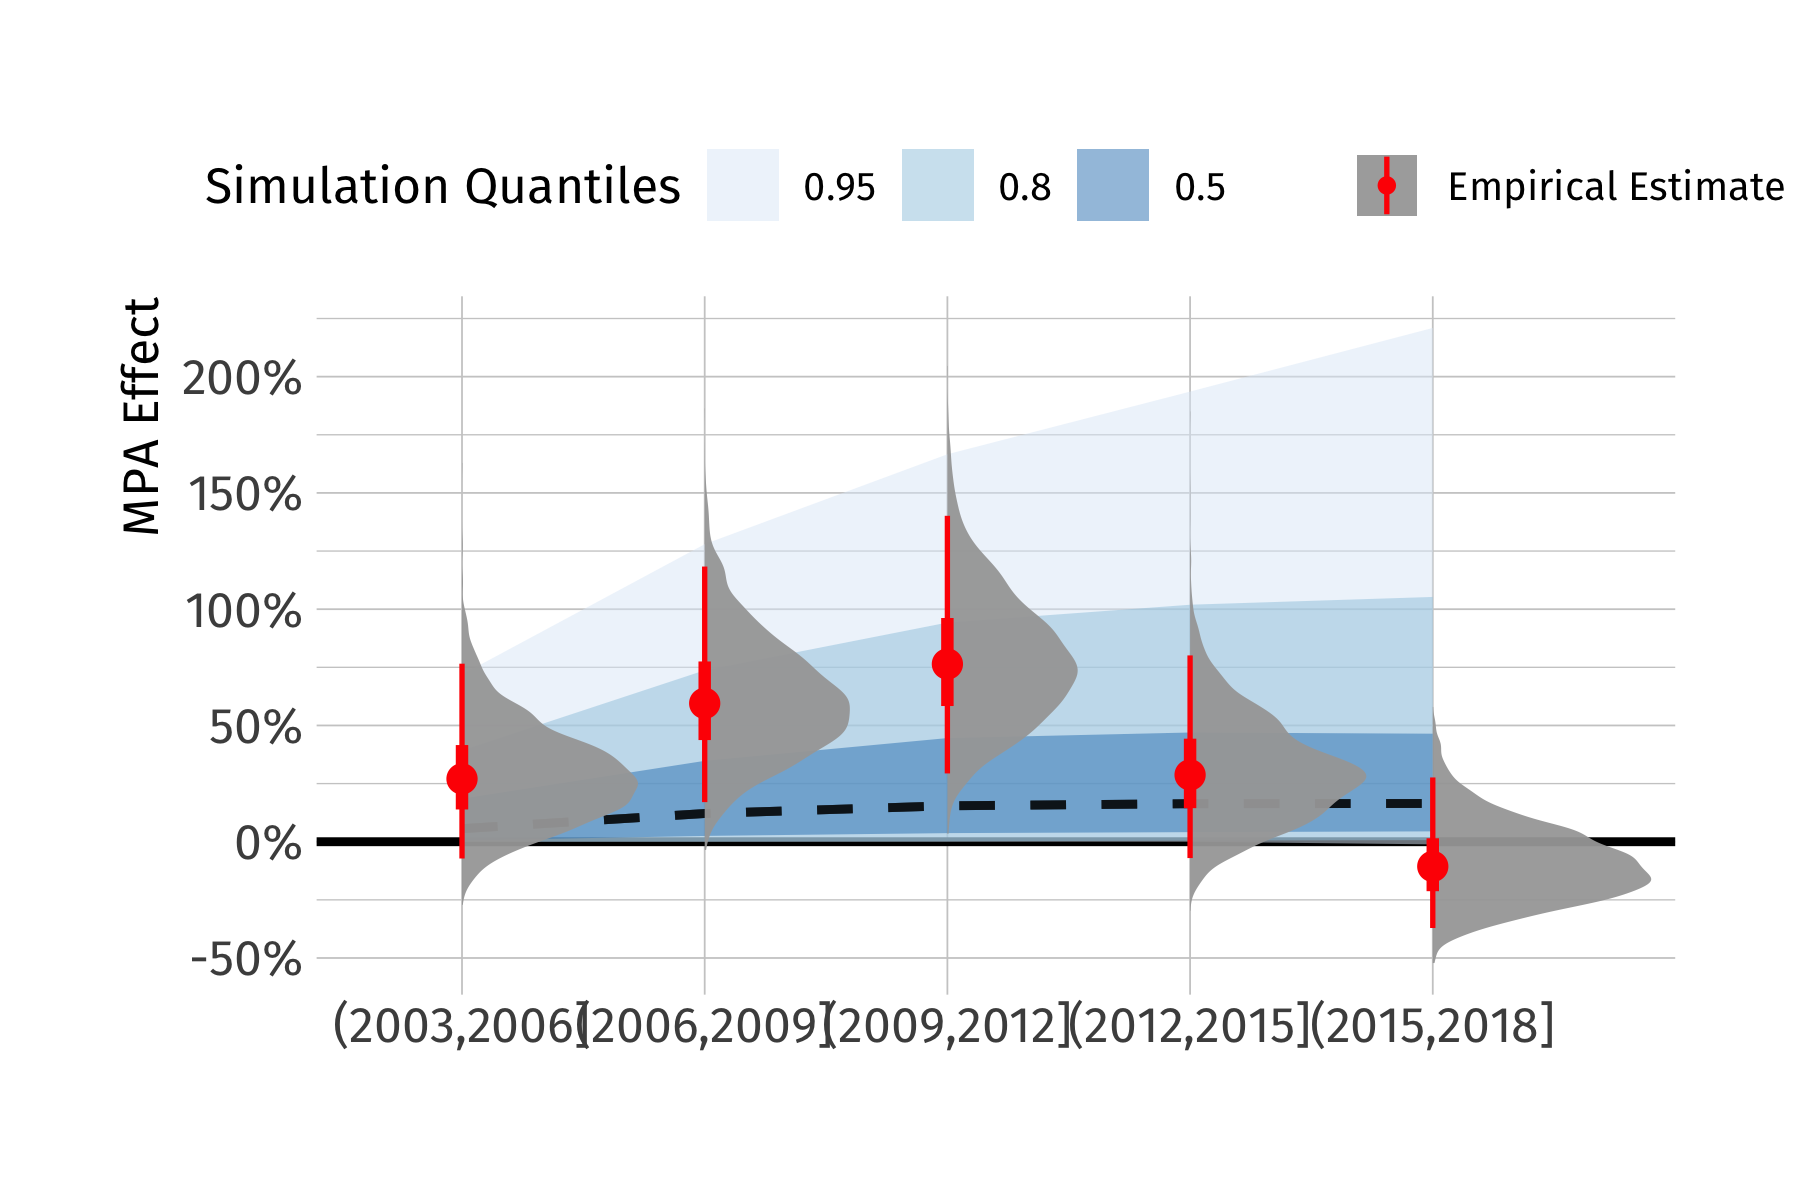
\includegraphics[width=.9\linewidth]{/Users/danovan/projects/regional-effects-of-mpas/documents/figs/mpa_effect_plot.png}
\textbackslash caption\{Results of difference-in-difference regression
estimating the regional effect of the northern Channel Island MPAs on
mean total biomass densities of targeted species (difference in mean
total biomass density of targeted species over time relative to expected
levels using non-targeted species as a control). Grey distributions show
90\%XX posterior probability distribution of estimated MPA effect; red
point is median estimated effect, thicker red section 50\% credible
interval, thinner red line 90\% credible interval). Blue distributions
in background show range of MPA effects produced by simulation model
tuned to reflect the dynamics of the Northern Channel Island MPAs (black
dashed line is median simulated value). Results are estimated in three
blocks, including years greater than or equal to left-hand value and
less than right-hand value.\} \label{mpa-effect}
\textbackslash end\{figure}\}

\hypertarget{discussion}{%
\subsection*{Discussion}\label{discussion}}
\addcontentsline{toc}{subsection}{Discussion}

\begin{enumerate}
\def\labelenumi{\arabic{enumi}.}
\item
  Why are the results from the channel islands important and what do
  they tell us
\item
  Put the channel islands results in context -
\end{enumerate}

Ideally then we want a control for broad environmental shocks to the
region that is independent of factors such as selection bias, biological
spillover, and fishing concentration.

\begin{enumerate}
\def\labelenumi{\arabic{enumi}.}
\item
  multiple lines of evidence
\item
  Theory before empirics
\item
  Patience
\end{enumerate}

The network of MPAs implemented in the Northern Channel Islands in 2003
provides an ideal opportunity to examine the regional effects of
protected area networks. This analysis is to our knowledge the first
empirical estimate of the regional effects of a large and iconic MPA
network on a broad assemblage of targeted fin-fish. Despite the well
enforced nature of these MPAs {[}xx{]}, and the presence of a rigorous
scientific monitoring program, we are unable to estimate a clear effect
of protection. While response ratios have targeted species have
increased over time, providing evidence of effective \emph{within MPA}
protection, these response ratios are on their own an unreliable
indicator of the regional conservation effects of the MPAs. Our
difference-in-difference regression estimates a high probability of
increasingly positive MPA effects over the first nine years of
protection, only to see these estimated gains reversed from 2012 to
2017. For the most recent time period, we can detect no clear positive
or negative regional effect of the Channel Island MPAs on biomass
densities of targeted fin-fish (Fig.@ref(fig:mpa-effect)).

How can we explain these results? The estimated effects from 2003 to
2014 are well in line with theoretical expectations given the species
and network in question. How might we explain the most recent results
though? One explanation may lie in fleet dynamics. Much of the
theoretical literature on MPAs assumes that all else being equal bigger
reserves produce bigger conservation gains ({\textbf{???}}). However, to
our knowledge all of these models simulate fleet dynamics through
assumptions about fishing mortality rates (e.g.~concentration of fishing
mortality (48)). The assumption of these models is that fishers
determine an amount off effort to exert, and distribute that effort
outside the MPA in response to some function.

An alternative and to our knowledge unexplored (in the context of MPAs)
fleet model though is a ``constant-catch'' strategy. Under this model,
fishers have a catch objective, and exert as much (or little) effort as
needed to achieve that objective. While a constant-catch greater than
MSY is not possible over the long-term under the assumptions of our
model, over the short-term a constant-catch scenario is not implausible.
Subsistence fisheries may use a constant-catch style policy over the
short-term, as they seek to ensure that their food needs are met. More
industrial fisheries may have pre-arranged agreements with buyers to
deliver set amounts of fish. Constant-catch dynamics might also occur in
fisheries with constraining quotas that are not updated after the
implementation of MPAs. Interestingly, when we simulated the effects of
MPAs under different fleet models, the ``constant-catch'' scenario stood
out as the only way for MPAs to actually produce a net conservation loss
(Fig.@ref(fig:XX)). While open-access fishing strategies can result in
``scorched earth'' scenarios where the only fish left are found inside
the reserve, across 94\% simulations the net effect of the reserves was
still positive. Under a constant-catch scenario though, fishers have to
fish much harder than before to get the same catch from a smaller part
of the population, reducing the size structure of the population and
subsequently causing net conservation loss under 70\% of our
constant-catch simulations.

While we do not have access to fine scale fishing data from the Northern
Channel Islands alone, reported catches for the species of interest in
the Santa Barbara region in fact exhibit an overall downward trend in
the years post reserve (see SI, XX). We can most likely rule a negative
MPA effect caused by a constant-catch fishing strategy then. What then
is another explanation for the recent downward trend in the estimated
MPA effects? We do not see evidence to reject the parallel trends
assumption of our difference-in-difference model in initial years of the
MPAs, and we do not detect any clear evidence of interaction between the
targeted and non-targeted species (e.g.~depressed levels of non-targeted
species as a result of predation from increased biomass densities of
targeted species, see Fig.SXX).

However, the Santa Barbara Channel experience a massive heatwave in XX.
The Channel Islands represent the warmest edge of the distribution of
many of the targeted species in our study. Conversely, many of the
represented non-targeted species are sub-tropical. As a result, we
hypothesize that the blob even of XX broke down the parallel trends
assumption between the targeted and non-targeted species in our study,
as the targeted species were more negatively affected by the warming
temperatures. This is supported by the fact that we observe similar
declines in targeted species both outside and inside the reserves
(Fig.XX). Assuming that the reserves are sufficiently well enforced and
large to protect targeted species biomass (an assumption supported by
the response ratio results), if the cause of recent declines was due to
increases in fishing pressure we would expect to see substantial
declines only in the fished areas (Fig. XX).

\includegraphics{ovando-regional-effects-of-mpas-v2_files/figure-latex/unnamed-chunk-5-1.pdf}

\begin{figure*}%[tbhp]
  \centering
  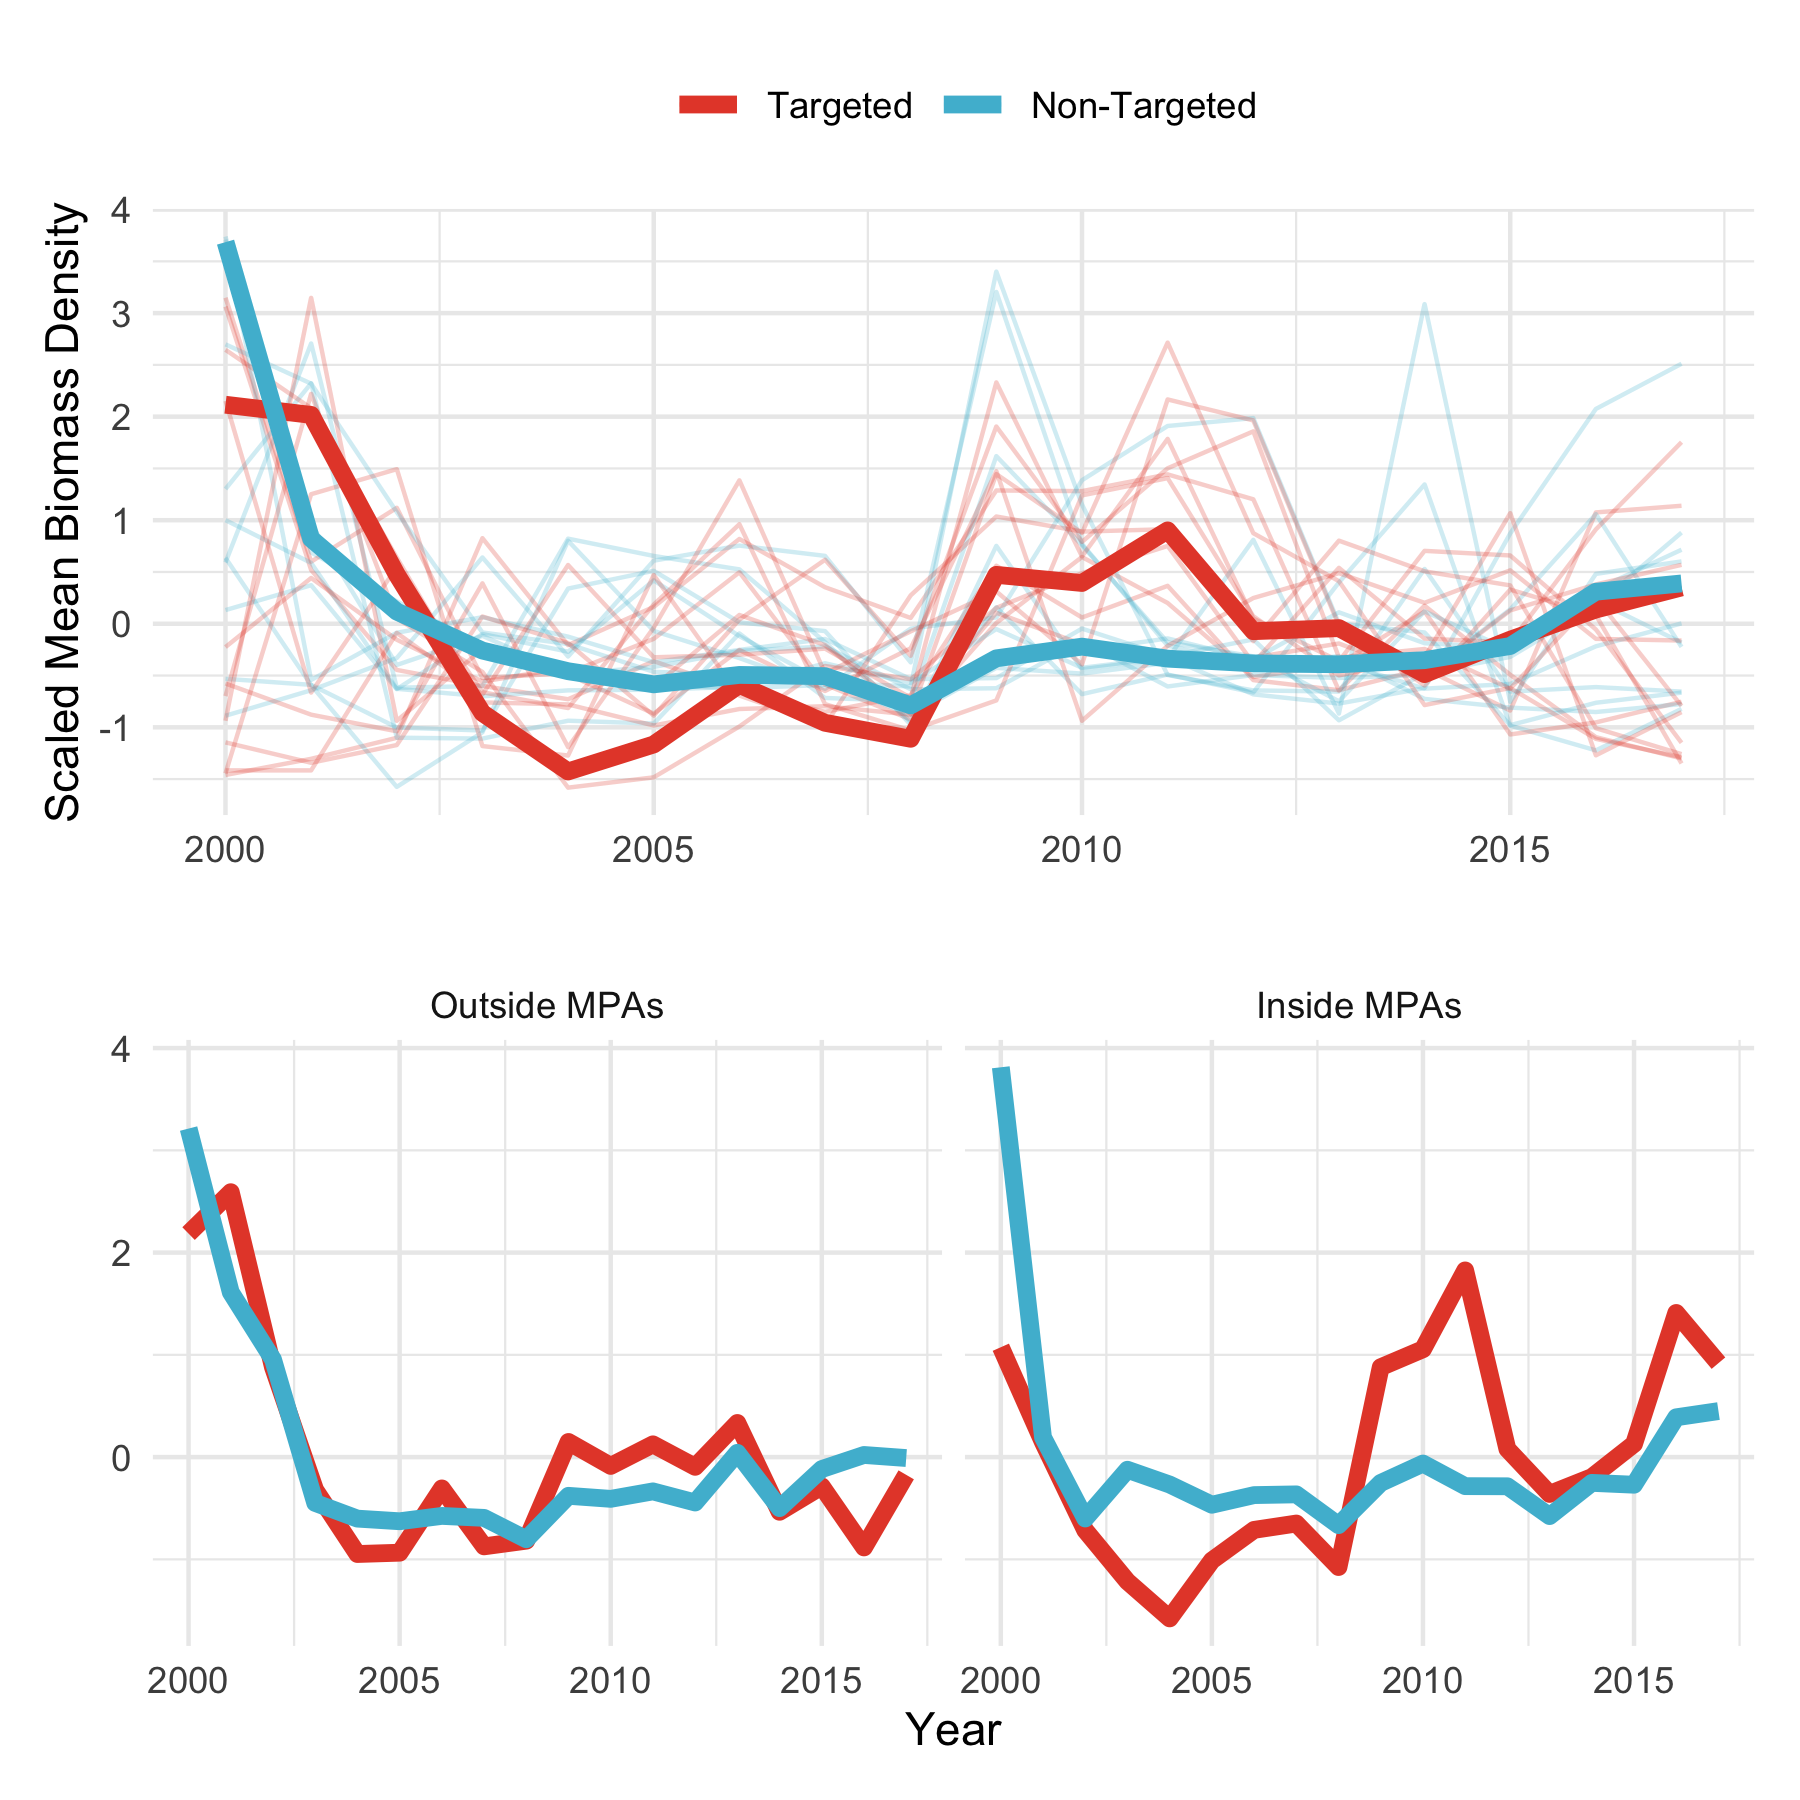
\includegraphics[width=.9\linewidth]{/Users/danovan/projects/regional-effects-of-mpas/documents/figs/raw_biomass_density_plot.png}
  \caption{Raw Biomass Trends}
  \label{mpa-effect}
\end{figure*}

\hypertarget{when-can-we-detect-the-effects-of-mpas}{%
\subsubsection{When Can We Detect the Effects of
MPAs?}\label{when-can-we-detect-the-effects-of-mpas}}

Containing a carefully designed, well-enforced, and well-studied MPA
network, The Channel Islands would seem at face value to be an ideal
location to study the regional conservation effects of protected areas.
The persistently high response ratios suggest that despite overall
decreases in targeted biomass densities inside and outside MPAs, the
MPAs may still be providing protection within their borders. But, as we
have shown here these response ratios are not necessarily a sign of the
magnitude of any regional effects. The difference-in-difference strategy
utilized here presents an alternative strategy, that while not without
its own strict caveats presents some potential improvements over
response-ratios as a means of estimating regional conservation effects.
While we estimate a highly uncertain but overall positive effect at
first, we are unable to detect a robust signal from 2012-2017. After 14
years of MPA protection we are left without a clear picture of the
effect of the Channel Island MPA network on biomass densities of
targeted fin-fish species.

Our simulation results suggest though that we should not be surprised by
this result. The Channel Islands MPAs cover approximately 20\% of the
waters in the Channel Islands, and while formal stock assessments are
not available for many of the targeted species in our analysis, what
evidence we have suggests that, as a group, these fish are on average
not heavily overfished. Some species, such as California sheephead and
blue rockfish were likely below target levels during the period (44,
45), but projections based upon the overall average response across all
species will likely suggest modest benefits even if a subset of species
could experience much larger population gains. Harkening back to our
simulations, we expect the average percentage difference in densities of
targeted species with and without MPAs to be modest
(Fig.\ref{fig:did-plot}). Effects of this size are likely to be
challenging to detect empirically given the large natural variation of
marine ecosystems (especially temperate reefs) and the observation error
inherent in infrequent annual survey programs such as those provided by
PISCO.

As an additional complication, our simulations difference-in-difference
model examine percentage changes in biomass densities. As an extreme
example, an increase in biomass densities from .2kg/m\textsuperscript{2}
to .4kg/m\textsuperscript{2} would be produce as a 100\% increase. While
a large percentage increase, this is a small change in absolute biomass
densities relative to the variance in the observation process itself
(see Fig.S1 for a companion to Fig.\ref{conservation-effects} scaled by
absolute population size). Beyond these challenges, the median estimated
age at sexual maturity for the targeted species included in this study
is 6 years, meaning that the span of this analysis represents less than
three generations of MPA protection for half of the the measured
species. Ongoing monitoring may yet reveal clearer effects. Analysis of
more rapidly growing and maturing species, e.g.~spiny lobster, may also
reveal clearer signals.

Given the natural variability of marine ecosystems, and the strong
challenges of obtaining accurate samples from oceanic environments, how
large of an effect would an MPA network have to allow a
difference-in-difference strategy such as this to be a reliable measure
of MPA effects? To provide guidance on this important question, we used
our bio-economic model to simulate data from a range of scenarios with
increasing MPA effect size, along with increasing degrees of observation
error and natural recruitment variation. As an added measure, we include
scenarios in which the sampled species go through recruitment regimes,
which may be positive for both targeted and non-targeted species, or
positive for non-targeted species and negative for targeted species. We
then used a simple Bayesian difference-in-difference regression on these
simulated data, and estimated the percent error between the estimated
and true MPA effect.

While unbiased across simulations, the difference-in-difference model
struggled severely when MPA effect sizes were less than 25\% and the
model was faced with observation and process errors
(Fig.@ref(fig:val-plot)). Even larger effect sizes commonly misestiamted
the true MPA effect by 50\% or more. Obtaining a mean absolute percent
error (MAPE) of 25\% or less across our simulated datasets required an
MPA effect of at least 30\%. This is merely an illustrative exercise,
omitting clearly critical factors such as detection probability and
sampling strategy. However, since nearly any omission which one can
think of would make an MPA effect harder to detect, not easier, these
results serve as a useful floor for the likely difficulty in estimating
MPA effects. In the context of the Channel Islands, given the potential
effect size produced by out simulation model these results suggest that
we might expect to be unable to detect a clear effect. XX need to think
about whether MAPE is the correct error here - maybe need something like
the variance of the estimator?

\begin{figure*}%[tbhp]
  \centering
  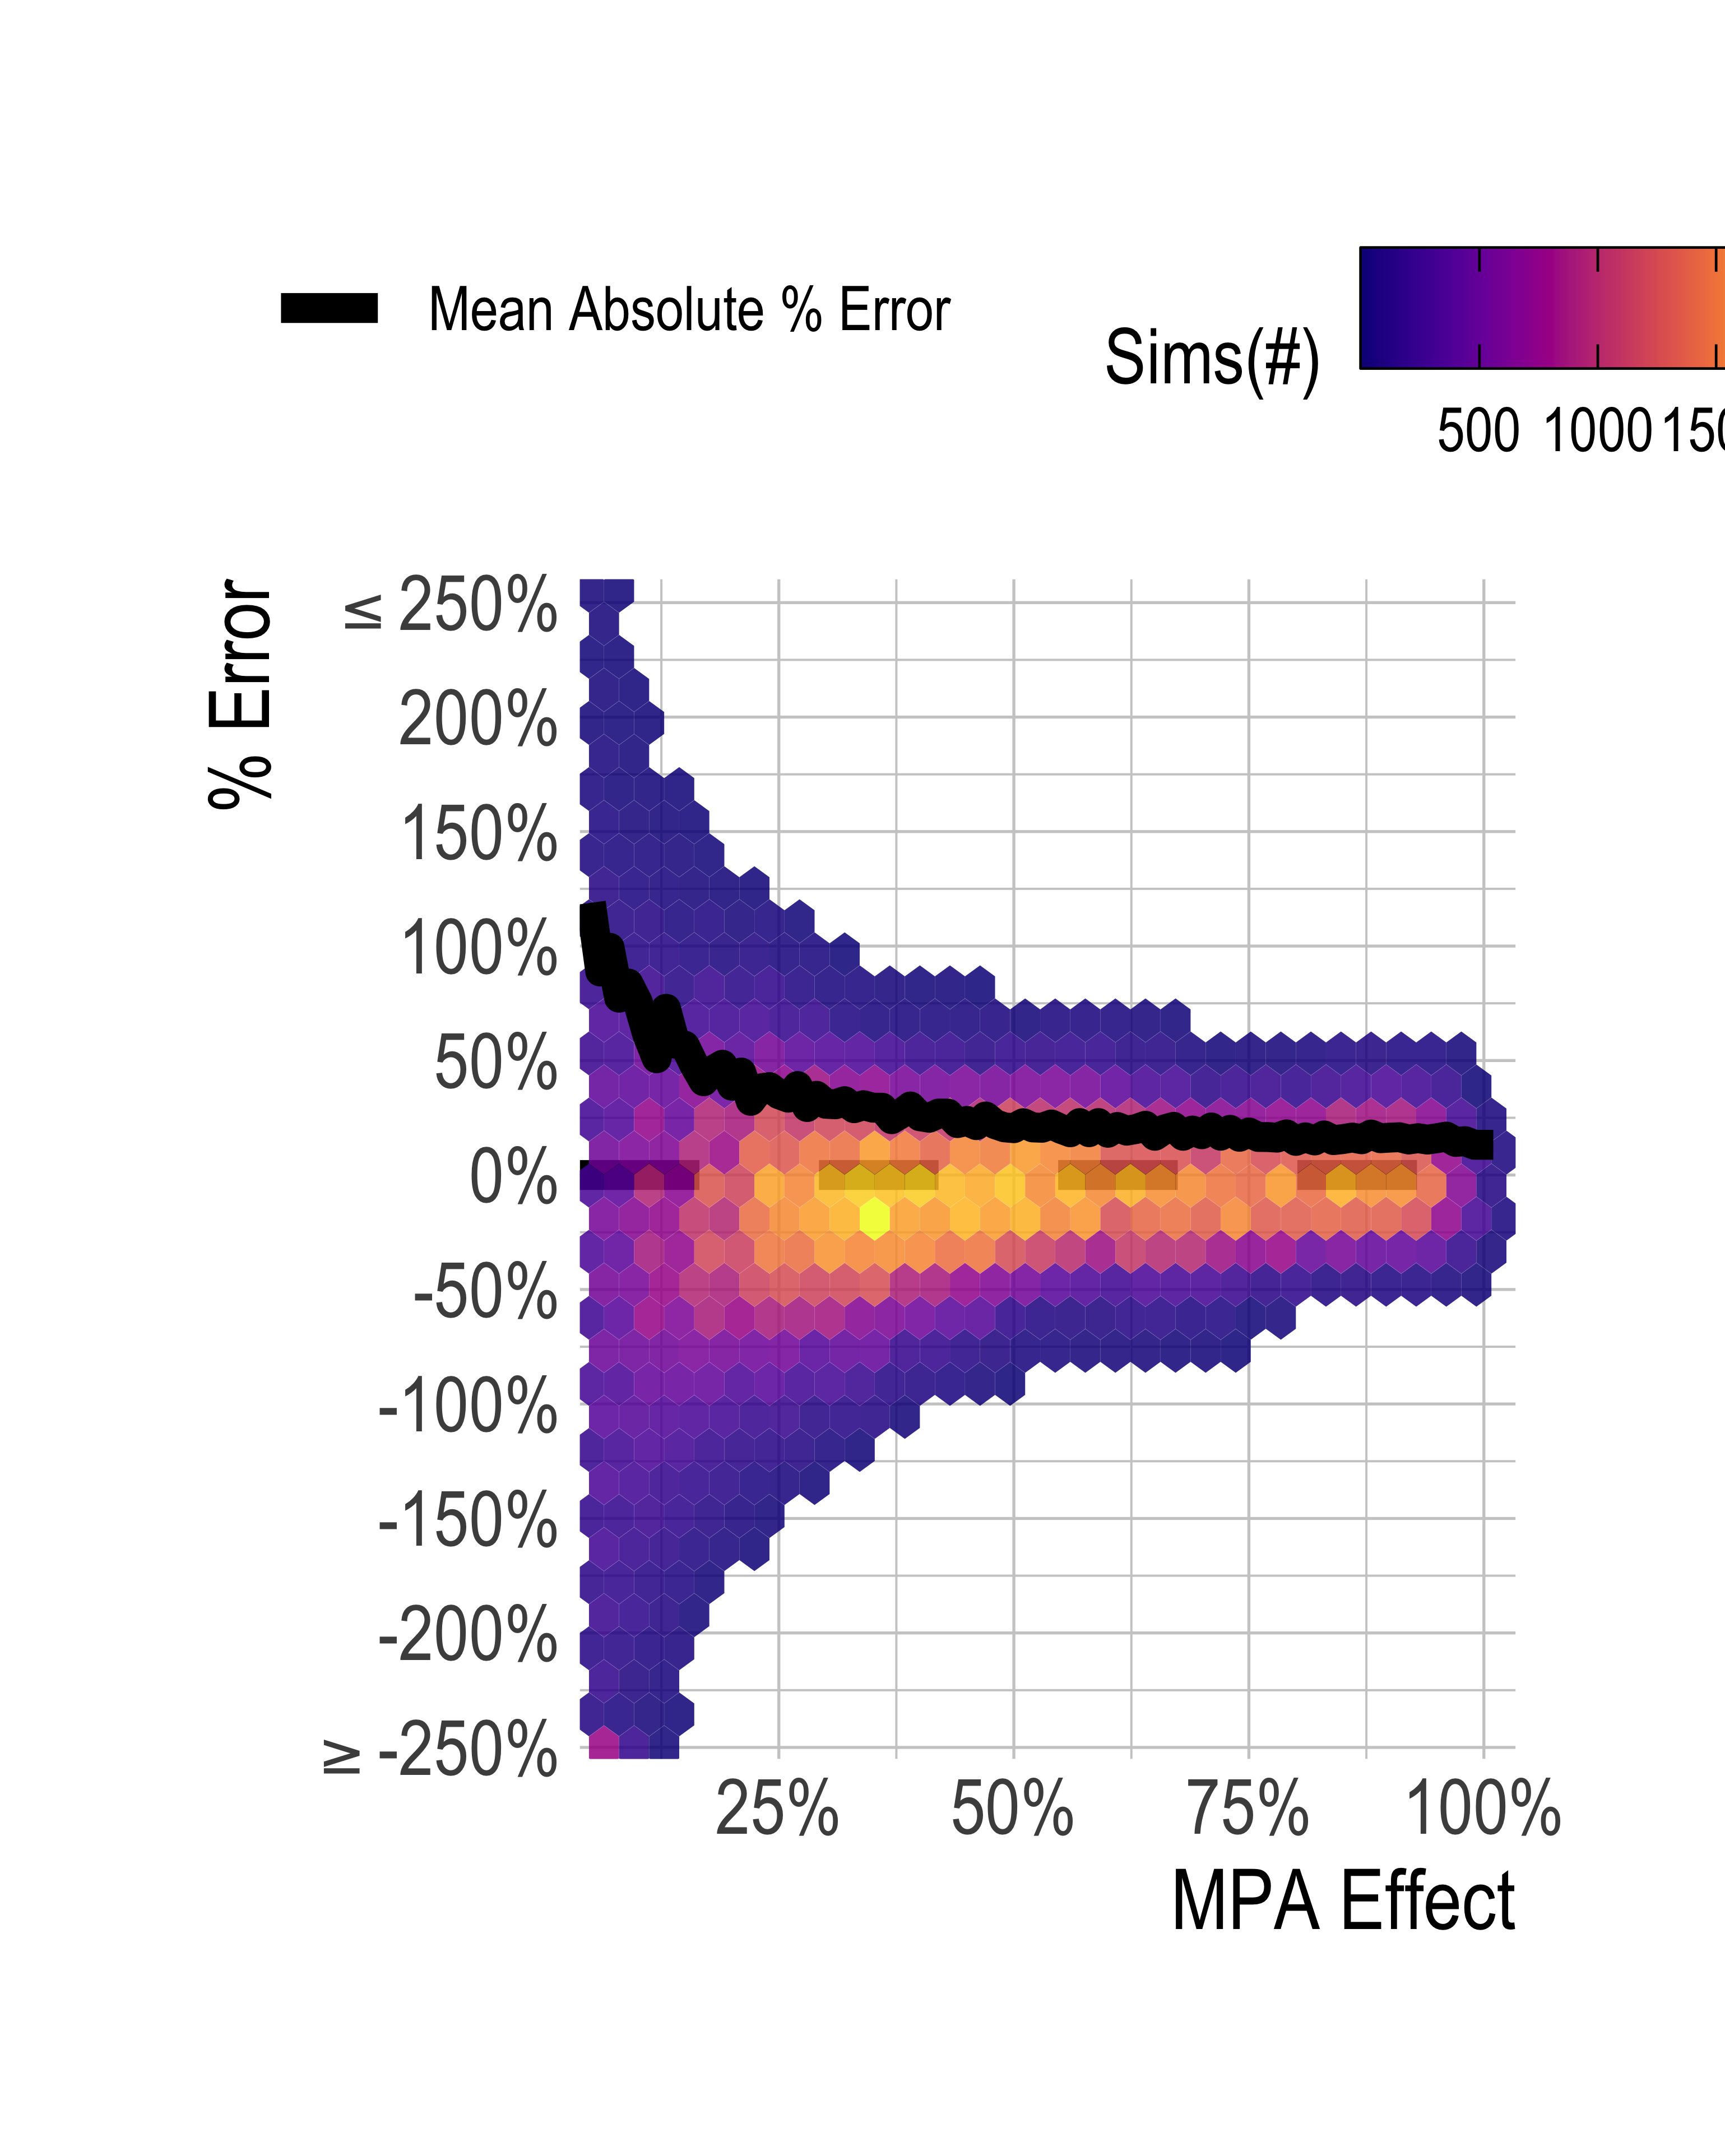
\includegraphics[width=.9\linewidth]{/Users/danovan/projects/regional-effects-of-mpas/documents/figs/validation_plot.png}
  \caption{Validation}
  \label{val-plot}
\end{figure*}

This finding begs an important question: when should we expect to see
MPA effects big enough to stand a reasonable chance of detection? To
address this, we simulated 9252 MPA scenarios across a wide range of
life histories, network designs, and fishing dynamics (see SI for a full
description of scenarios). Using these simulations, we can consider what
we might expect the regional effects of an MPA network to be under a
range of plausible circumstances.

Suppose that we are willing to tolerate a MAPE of 25\%. Two of the most
critical drivers of MPA performance are the size of the MPA and the
degree of fishing pressure. Looking across these two variables, our
simulations suggest if the MPA network covers 25\% or more of a species
range and/or pre-MPA depletion is greater 60\% we might expect an effect
size with a reasonable chance of detection. While recently some
extremely large MPAs have been enacted that may indeed reach into the
higher levels of MPA coverage, for near-shore commercial fin-fish many
MPA networks are likely to cover areas more in line with the Channel
Islands (20\%) (Fig.@ref(fig:XX)-A).

These initial simulation results would seem to suggest some rather
simple rules of thumb: put an MPA of sufficient size on a at least
somewhat overexploited population and one can expect large and
potentially detectable results. However, as we discussed earlier, the
MPA literature highlights a large number of variables beyond simply size
and fishing pressure that can affect performance. To address this, we
can examine the variability in expected MPA effects across each of the
two major axes (pre-MPA depletion and MPA size) (Fig.@ref(fig:XX)-B). As
both MPA size and pre-MPA depletion increase, the potential for a large
MPA effect increases. However, we see that for both variables, even at
extremely large or extremely small values a wide range of MPA effects
were possible, though as we might expect this effect of pre-MPA
depletion, in other words fishing pressure were much clearer: it is hard
for an MPA to have a massive effect when the stock is not heavily
fished.

To put these results into further context, the FAO estimates that 7\% of
the worlds fisheries with status estimates fall into the relatively
unexploited category (roughly depletion less than 50\%), 60\% fall into
the fully fished category (roughly depletion 50\%-70\%), and 33\% fall
into the heavily fished category (roughly depletion greater than 70\%)
(52), though works that include a broader range of fisheries estimate
that 50\% or more of stocks to fall into the heavily fished category
(53, 54). Taken together then, the regional effects of MPA networks
covering 25\% or less of a species range may be difficult to detect in
many placed with already well-managed fisheries, while for that size we
might expect clearer effects in less-managed locations (though that of
course ignores the complication of compliance with MPA regulations).
Within these broad guidelines though a wide range of outcomes are
possible: as a starting place users can use the bio-economic MPA
simulation model developed for this paper to explore potential outcomes
for specific MPAs using an interactive web application available at
\href{https://danovando.shinyapps.io/simmpa/}{danovando.shinyapps.io/simmpa}.

\begin{figure*}%[tbhp]
  \centering
  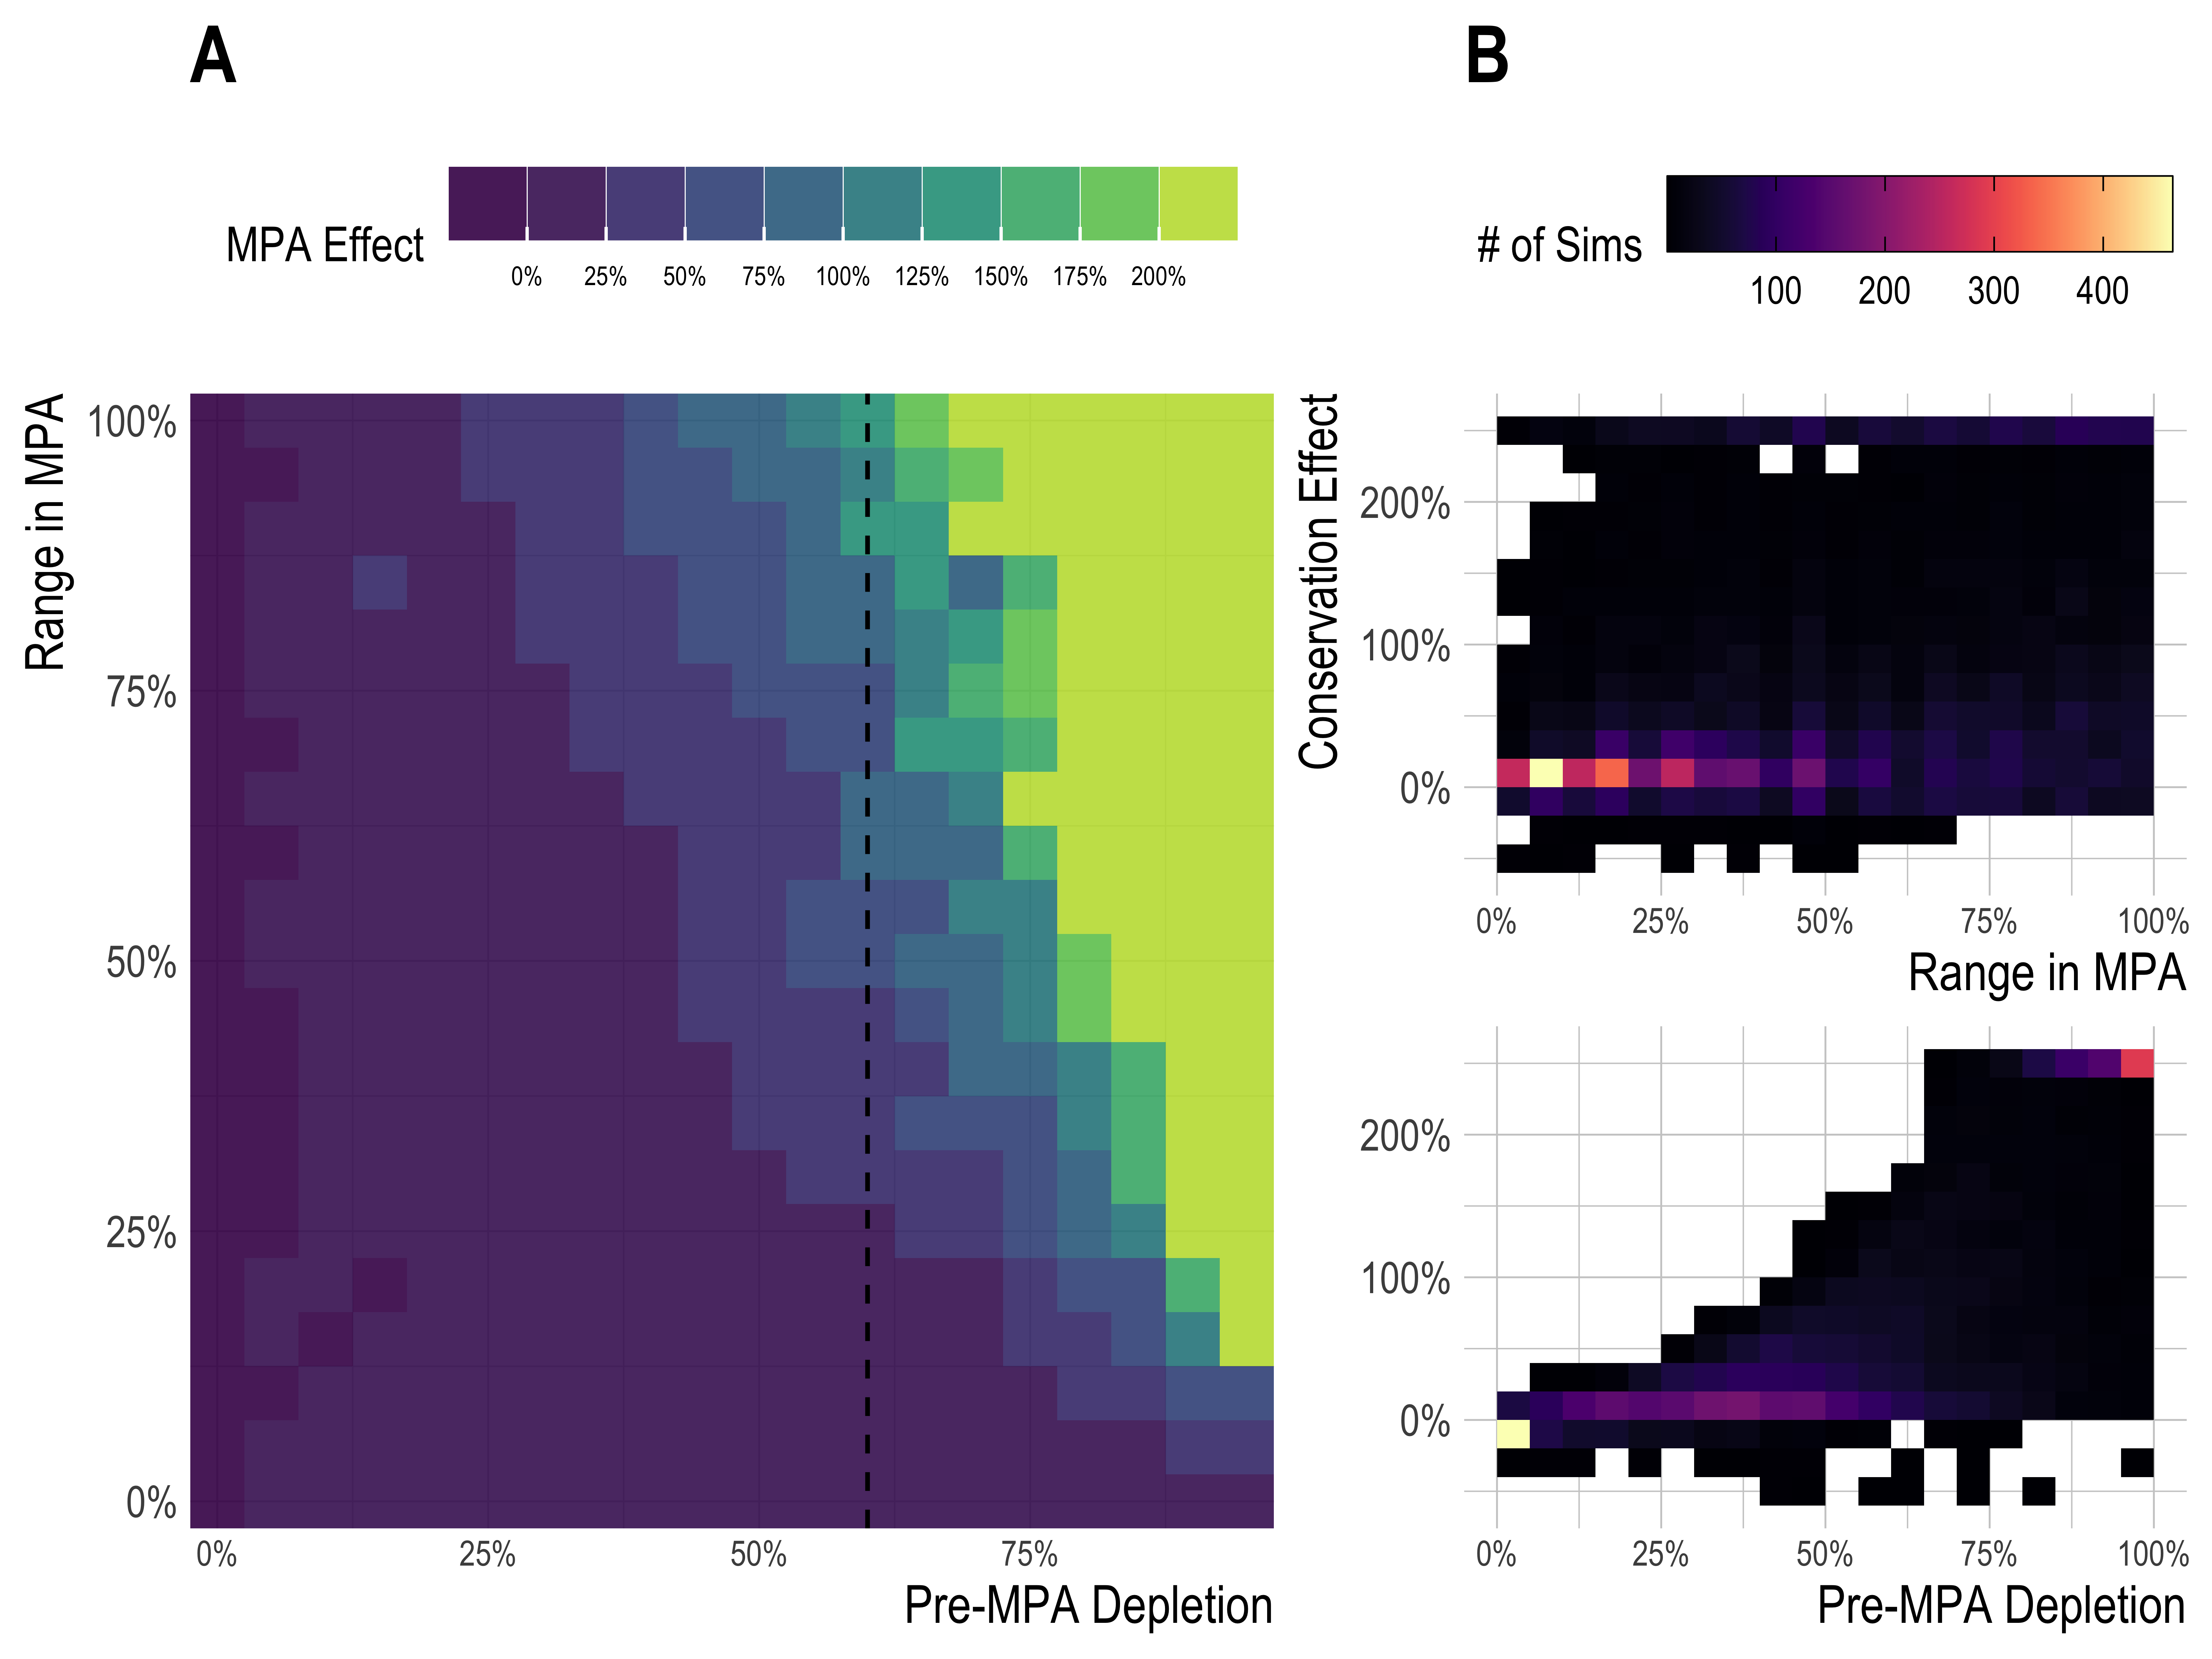
\includegraphics[width=.9\linewidth]{/Users/danovan/projects/regional-effects-of-mpas/documents/figs/expected_mpa_effect.png}
  \caption{Expectation}
  \label{expect-plot}
\end{figure*}

\hypertarget{conclusion}{%
\subsection*{Conclusions}\label{conclusion}}
\addcontentsline{toc}{subsection}{Conclusions}

MPAs are an important part of the marine resource management toolbox.
Under ideal circumstances they can protect individual species and
ecosystem linkages, while supporting local economies through tourism and
fishing opportunities. One rationale for the expansion of MPAs is that
they will deliver net conservation benefits both inside \emph{and
outside} their borders. To date, this assumption is insufficiently
tested, and this is the focus of our paper. Our results show that
regional conservation benefits of MPAs are highly context dependent and
in many circumstances, are likely to be small enough that they are
nearly impossible to detect empirically. Indeed, this is exactly what we
found in our empirical case study from the Channel Islands, California,
USA.

What do our results imply about the future of MPA science? Our
simulation model is by no means exhaustive (for example it ignores
features such as species interactions, habitat effects, and climate
feedback), but captures many of the core factors theorized to affect MPA
performance. Our results show that while attributes such as MPA size and
fishing pressure are important factors in determining the effects of
protection, local fleet dynamics and the movement rates of adult fish
can dramatically affect the outcomes of protected areas as well
(Fig.\ref{conservation-effects}). Far from being a simple tool with
clear outcomes, the effects of MPAs can be highly context dependent,
requiring - we would argue - a bio-economic model of at minimum the
complexity presented here to help communities design and set
expectations of MPAs at the tactical level. While users may not be able
to parameterize every aspect of a model such as that presented here,
working with stakeholders to visualize the implications of, for example,
different fleet responses to MPA implementation is a critical step in
MPA design. Readers can use our simulation model to explore the effects
of MPAs through an interactive web application available
\href{https://danovando.shinyapps.io/simmpa/}{here}.

Once simulation models have been used to help design an MPA, how can
users evaluate whether it is achieving their objectives? Response ratios
are commonly used as evidence for conservation outcomes of MPAs; (5) and
(55) present meta-analyses of hundreds of such studies. These results
often find massively higher densities and biomass inside MPAs than
outside (5). But as suggested in (47) and (49) and further demonstrated
here, without careful attention to the design of control sites
(accounting for example for the displacement of fishing effort by MPAs),
response ratios may be highly unreliable estimators of regional MPA
effects. When MPAs affect nearby control sites used in response ratios
through biological spillover or concentration of fishing effort, it is
entirely possible to for MPA to produce massive response ratios while
simultaneously having minimal effects on the actual populations
partially protected by the MPAs. As (49) suggests, there are many
potential alternatives for estimating the effects of MPAs that better
account for the challenges of causal inference (though that may be more
data-intensive). We applied one such approach here (a
difference-in-difference estimator), and yet were still unable to reach
robust conclusions as to the effect of MPAs on the density of targeted
species in the Channel Islands, due to the likely small size of the true
effect relative to the strength and variability of environmental
drivers.

While this does not mean that all MPAs will face similar challenges in
estimating their effects, our results in the rigorously studied and
iconic Channel Islands Marine Protected Area network make clear that in
many instances empirically detecting a clear regional effect of MPAs may
not be possible. How then should stakeholders go about adaptively
monitoring and managing MPAs? Simulation modeling can help inform the
range of effect sizes that may be expected, and monitoring programs can
perhaps be tuned to focus on the species groups that have the highest
chance of a detectable effect size (56). Expanding data collection to
include robust monitoring of spatio-temporal fleet dynamics may help
assess the validity of control sites used in response ratios, support
the direct inclusion of these fleet dynamics into statistical models,
and allow managers to take into account potential negative interactions
between MPAs and fleet dynamics such as those that may occur under
constant-catch dynamics. Whenever possible monitoring programs should be
implemented prior to MPA implementation to provide a pre-treatment
benchmark. Non-equilibrium analyses also help set expectations for
effect sizes over time (56). Educating communities about the challenges
of estimating the effects of MPAs can help set expectations, so that a
lack of a clear effect is not necessarily viewed as a failure of the
program, or a cause for premature adaptation of the network, but rather
considered in the context of reasonable expectations for the MPAs in
question. While this paper has focused on the conservation outcomes of
MPAs, future work must also address the challenge of predicting and
estimating the fishery impacts of protected areas.

As the number and size of global MPA networks increase, it is critical
that we both set appropriate expectations for their outcomes, and plan
how we will monitor the performance of these protected areas over time.
While the history of MPA science has made important strides in helping
us understand the dynamics of protected areas, the future of MPA science
must directly tackle the challenge of evaluating the performance of
these MPAs at the regional scale, and adapting their design as needed to
best achieve objectives. Commonly employed metrics such as response
ratios may be applicable in some circumstances, but can have severe
shortcomings as metrics of regional conservation effects. Dependence on
unreliable estimators of MPA effects may lead to stakeholders
incorrectly attributing negative environmental shocks as MPA failures,
or interpreting data arising from scorched-earth fishing outside MPAs as
a conservation success. Bio-economic modeling can help frame community
expectations, reducing the potential for a reduction in support if
unrealistic conservation or fishery expectations are not realized.
Statistical approaches that explicitly address complications such as the
spatial spillover effects of MPAs (such as the difference-in-difference
approach used here) may give users an improved understanding of the
performance of their MPAs, but even they may struggle when expected
effect sizes are small. Clearly communicating what we should expect, and
what we can detect,m from MPAs is critical in ensuring that MPAs play
effective roles in fisheries management and marine conservation.

\hypertarget{materials-and-methods}{%
\subsection{Materials and Methods}\label{materials-and-methods}}

We present here critical characteristics of our simulation model and
regression approach. Further details can be found in the Supplementary
Information. All analysis were conducted in R (57). Our main
difference-in-difference model was fit using Stan (58) using the
\texttt{rstanarm} package ({\textbf{???}}). Code needed to replicate
results can be found
\href{https://github.com/DanOvando/regional-effects-of-mpas}{here}.

\hypertarget{simulation-model}{%
\subsubsection{Simulation Model}\label{simulation-model}}

Our bio-economic model simulates the effect of MPAs on a spatially
explicit age-structured representation of a single species. Readers can
explore the functionality of the model using an online tool available
\href{https://danovando.shinyapps.io/simmpa/}{here}. See Table.S1 for a
complete description of simulation states. The model consists of 25
patches with wrapped edges (picture the waters around a circular
island). For any one simulation we randomly pull a species and its
associated life history from the \texttt{FishLife} (41) package in R. We
pair these data with randomly selected values between 0.6 and 0.95 for
Beverton-Holt steepness (59), as well as larval and adult dispersal
rates. We also randomly assign whether adults have density dependent
movement, as well as one of three potential types of density dependence
(60):

\begin{enumerate}
\def\labelenumi{\arabic{enumi}.}
\item
  Local density dependence: Density dependence occurs independently in
  each patch, and recruits then disperse to nearby patches
\item
  Global density dependence: Density dependence is a function of the sum
  of spawning biomass across all patches, and recruits are then
  distributed according to habitat quality
\item
  Post-dispersal density dependence: Larvae are distributed throughout
  the system, and then density dependence occurs based on the density of
  adult biomass at the destination patch
\end{enumerate}

We allow for three potential siting strategies for MPAs. In the first,
MPAs are randomly placed. In the second, we assume that MPAs are placed
in preferentially better habit (unfished recruitment is four times
greater inside MPA locations). In the third, we allow for scenarios in
which MPAs are placed in hotspots of larval dispersal. In this scenario,
patches in which MPAs will be placed have larval dispersal rates four
times greater than patches that do not become MPAs.

Each simulation is randomly assigned a fleet model of the form

\begin{enumerate}
\def\labelenumi{\arabic{enumi}.}
\item
  Open access: fishing effort changes in response to
  profit-per-unit-effort
\item
  Constant effort: total fishing effort is constant over time (unless
  altered by MPA displacement model)
\item
  Constant catch: the fleet exerts as much effort as need to achieve a
  target catch
\end{enumerate}

This fleet model is paired with a gear selectivity ranging from .1 to
1.5 of the length at 50\% maturity for the species in question, and the
fleet model is tuned to achieve a target fishing mortality relative to
natural mortality ratio at equilibrium.

Along with the fleet dynamics model, each simulation is assigned a
random fleet dispersal scenario: uniform dispersal (where the total
effort of the fleet is divided evenly among all open patches), catch
dispersal (where the total effort of the fleet is divided according to
the catchable biomass in each available patch), and profit dispersal
(where the total effort of the fleet is divided according to the profit
per unit effort in each available patch).

Lastly each simulation is assigned an MPA scenario, defined by the
number and size of MPAs, the placement of those MPAs, and the year that
the MPAs are put in place. Each simulation starts the population off at
unfished equilibrium and then beings to apply the fleet model. The MPAs
are then placed during the randomly selected start year, allowing some
runs to explore how the early dynamics of the MPA play out when the
fishery and population they are placed on is not already at equilibrium.
Fishing effort in displaced by MPAs can either concentrate outside or
leave the fishery. Each simulation is run to equilibrium with and
without the selected MPA strategy (holding all else constant). We then
measure the difference in biomass densities each time step in the
scenario with and without the MPAs to calculate the conservation and
fishery effects of the MPAs over time.

\hypertarget{difference-in-difference-regression}{%
\subsubsection{Difference in Difference
Regression}\label{difference-in-difference-regression}}

\begin{figure}%[tbhp]
  \centering
  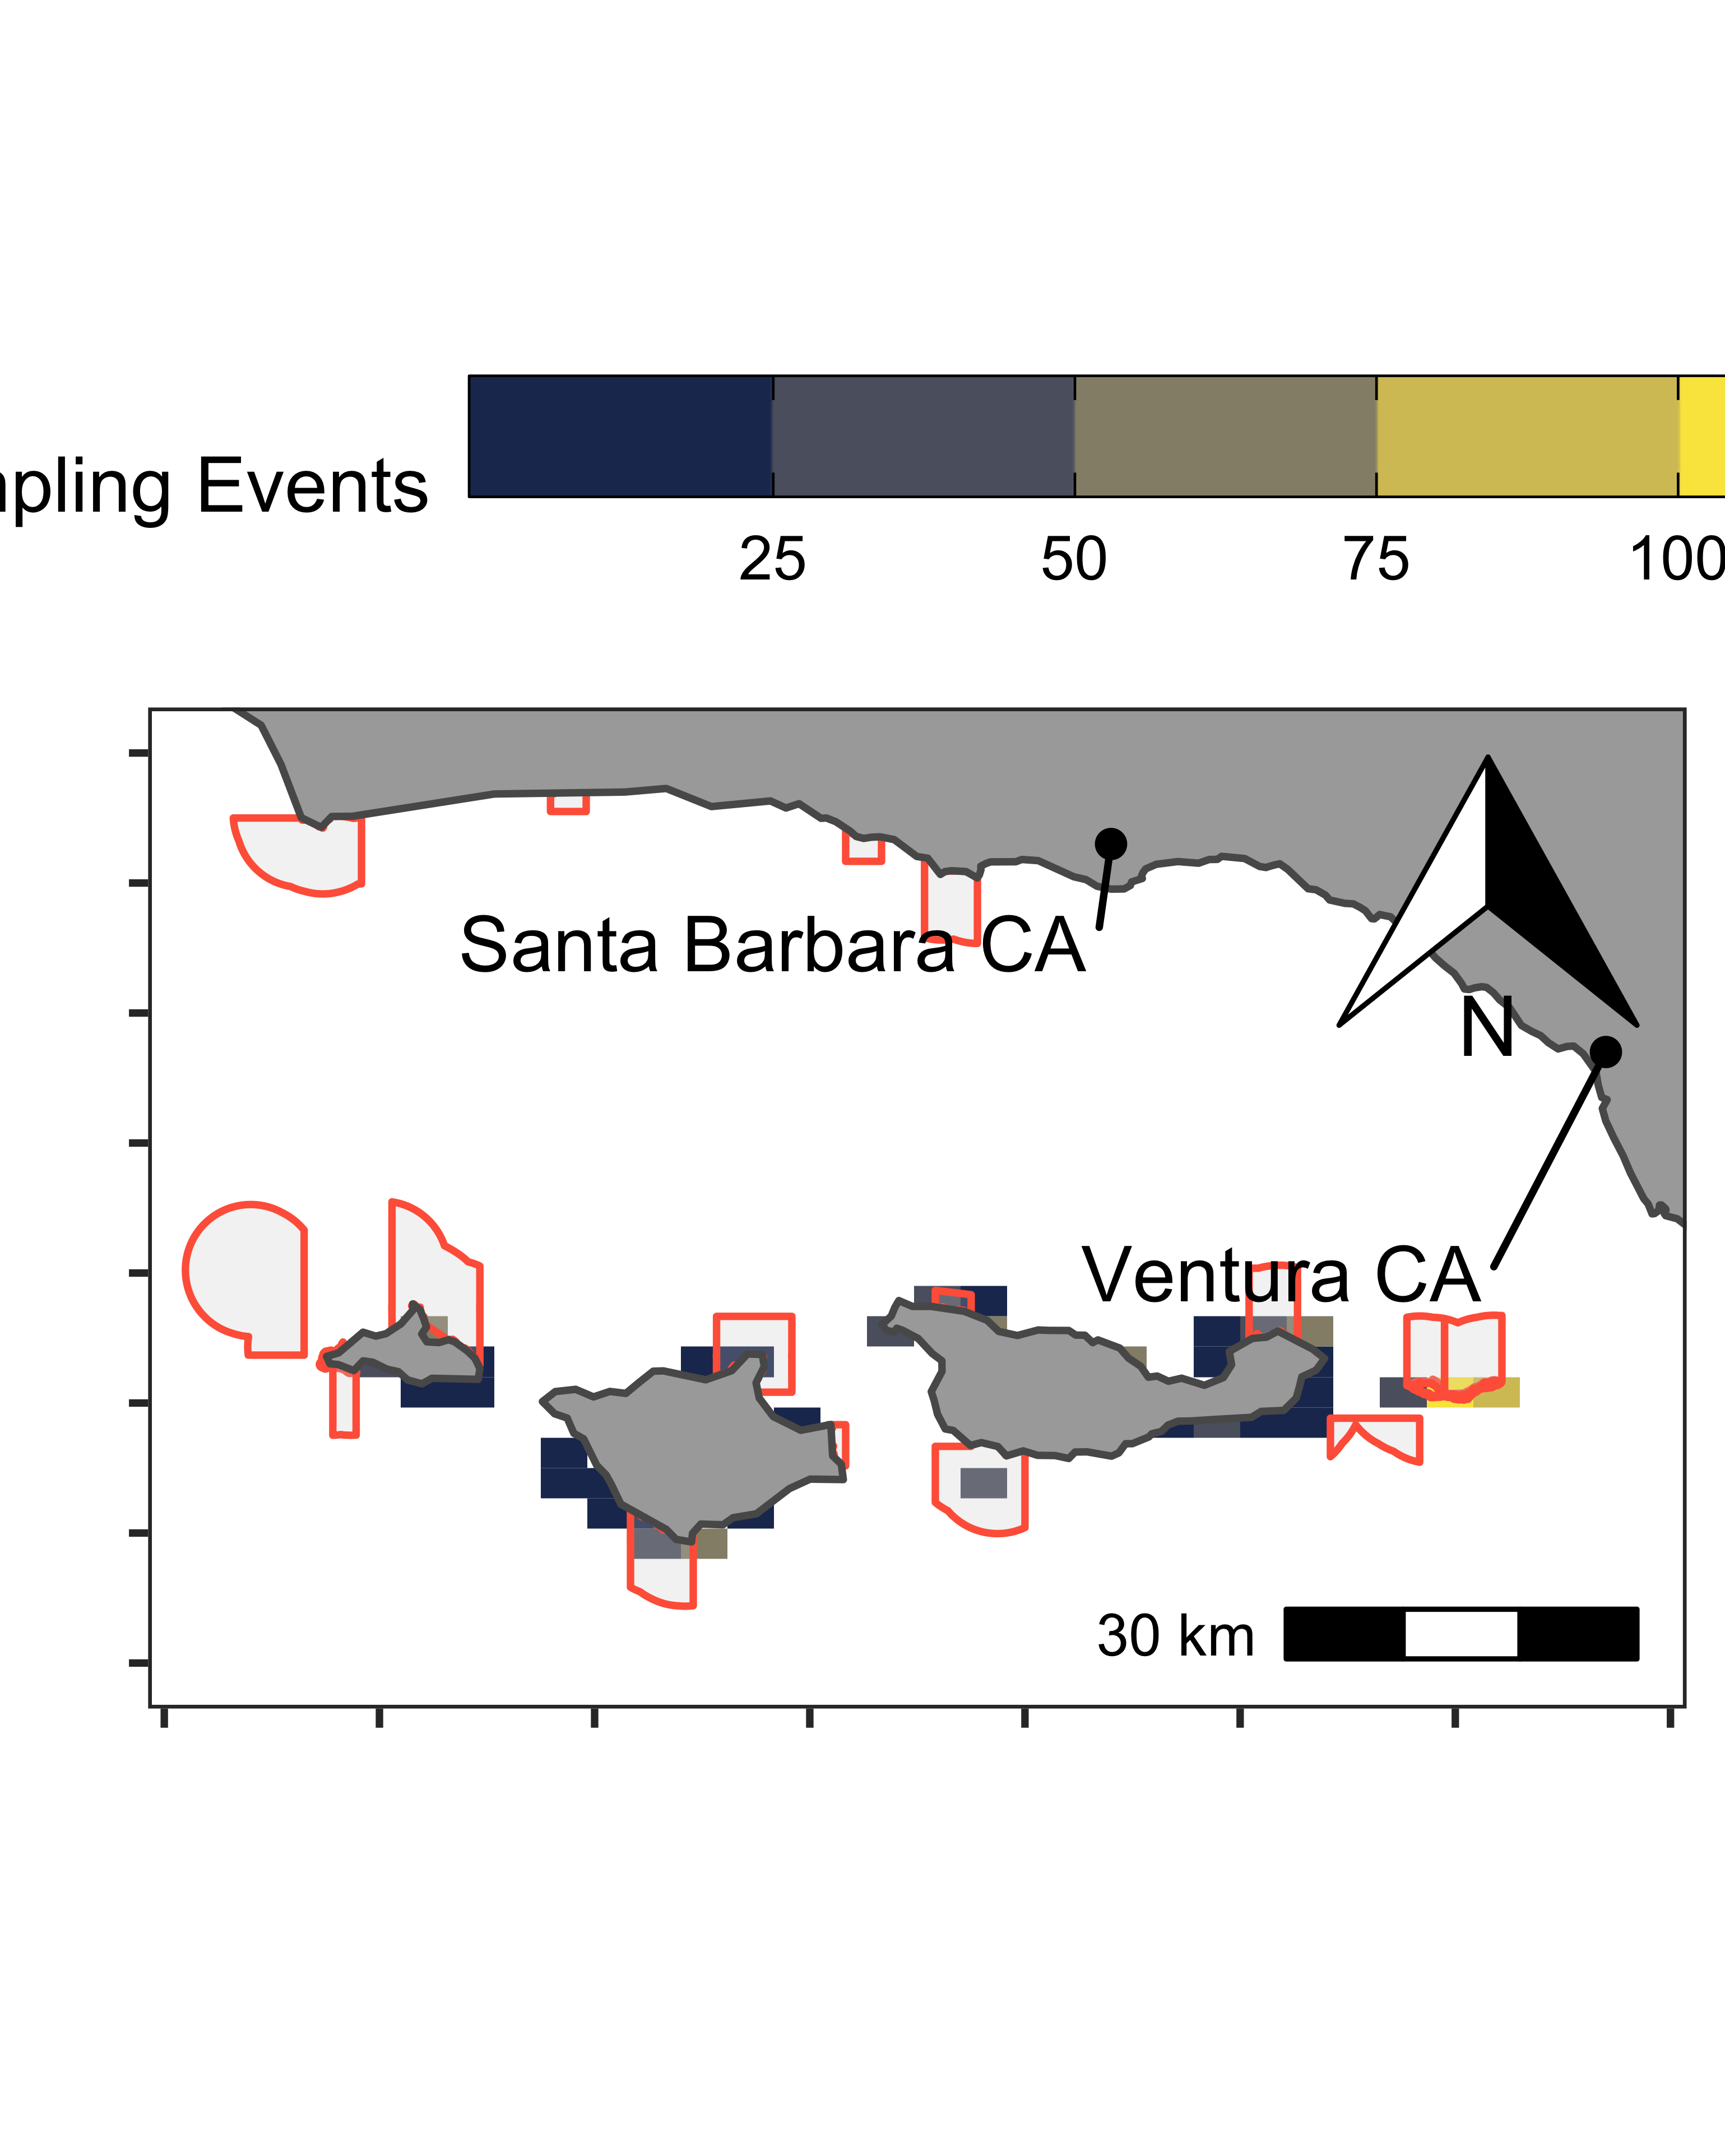
\includegraphics[width=1\linewidth]{/Users/danovan/projects/regional-effects-of-mpas/documents/figs/sample_location_plot.png}
  \caption{Map of PISCO sampling locations within the the Channel Islands National Marine Sanctuary, California, USA. Grey boxes indicated MPAs, points sampling locations, with color representing whether the site is inside an MPA (blue) or not (red)}
  \label{channel-islands}
\end{figure}

The difference-in-difference model used empirical kelp forest survey
data from the Partnership for Interdisciplinary Studies of Coastal
Oceans (PISCO) monitoring in the Northern Channel Islands. A network of
MPAs covering approximately 20\% of the islands' waters was put in place
in 2003 as part of the California Marine Life Protection Act (MLPA) (see
(22), (23), (24), and (25) for information on the creation of the MLPA).
PISCO conducts visual SCUBA surveys at a large number of rocky-reef and
kelp forest sites inside and outside of MPAs throughout the Channel
Islands, producing estimates of densities of fishes that are both
targeted and non-targeted by fishing
(Fig.\ref{channel-islands}-\ref{pop-trends}). . The details of the
monitoring program are described in XX

The key assumptions of the difference-in-difference model are that a)
within the time-frame of the model there are no significant interaction
effects between the targeted and non-targeted species (which in fact we
do not detect, see SI), and b) that in the absence of the MPAs both the
targeted and non-targeted groups of species would have exhibited similar
trends in densities. The advantage to this approach is that given the
time-frame of the model (14 years with MPAs), we believe that spillover
effects of MPA placement on the non-targeted species are likely to be
much less severe than the effects of biological spillover and fishing
concentration that may bias the performance of estimators such as a
response ratios.

The regression amounts to estimating the pre-post MPA difference in the
biomass densities of targeted species net the same difference for
non-targeted species in the Channel Islands.

The simplified form of this model is XX adjust to GAMMA glm

\begin{equation}
  d_{i} = Gamma(e^{\beta_0 + \beta_1T_{i} +  \beta_2MPA_{i} + \beta_{3}T_iMPA_i},shape, scale)
\label{eq:did}
\end{equation}

where \(d_i\) is the biomass density at observation \emph{i}, \emph{T}
indicates whether the observation \emph{i} is for a targeted (\(T = 1\))
or non-targeted (\(T = 0\)) species, and \emph{MPA} marks whether
observation \emph{i} is in a pre MPA (\(MPA = 0\)) or post MPA
(\(MPA = 1\)) state. is a vector of coefficients for additional control
variables in matrix \emph{X} such as water visibility and observer
experience. Under the assumptions of this model, \(\beta_3\) is the
causal effect of the treatment (\emph{MPA}) on the treated (targeted
species). The shape and scale parameters of the Gamma distribution are
estimated as well. See SI for further details of the estimation model.

We briefly assess two of the most critical assumptions of this model
here: that the treated and non-treated groups have parallel trends, and
that the effect of the treatment on the treated does not tangentially
affect the untreated. While the parallel trends assumption cannot be
formally proven, we can examine its validity using the data from the
years before the MPAs were put in place in 2003. We do not detect any
significant differences in the trends of the biomass densities of the
targeted and non-targeted species in the years before the MPAs. XX

With regards to the second assumption, all of the species in this
empirical analysis exist within an ecosystem, and as such affect each
other through mechanisms such as predation, competition, and habitat
modification. We find it unlikely that these effects have had enough
time to manifest in a meaningful way in the 13 years of post-MPA data
used in our analysis (61, 62).

We used convergent cross mapping (CCM), in the manner of (63), to test
for the possibility of the trophic cascades biasing our results.
Generalizations of Takens' theorem indicate that if two variables are
part of the same dynamic system, their individual dynamics should
reflect their relative causal influence. Convergent cross mapping (CCM)
tests for causation by using the attractor/manifold built from the time
series of one variable to predict another (hence the ``cross-mapping'').
CCM then allows us to test for causal relationships in the timeseries of
densities of targeted and non-targeted species. Our results found no
significant cross-mappings between targeted and non-targeted species,
indicating that while clearly there are interactions between these
groups on some level, the effects within the timespan of the data are
not pronounced enough to be of concern to our results (see SI for
additional information in CCM testing). However, the longer MPAs are in
place, the greater the possibility that substantial species interactions
that can affect use of non-targeted species as a control may arise.

~ ~ ~

\hypertarget{refs}{}
\leavevmode\hypertarget{ref-johannes1978}{}%
1. Johannes RE (1978) Traditional Marine Conservation Methods in Oceania
and Their Demise. \emph{Annual Review of Ecology and Systematics}
9(1):349--364.

\leavevmode\hypertarget{ref-iucn1976}{}%
2. IUCN (1976) \emph{IUCN yearbook, 1975-76 : Annual report of the
International Union for Conservation of Nature and Natural Resources for
1975 and for January-May 1976}.

\leavevmode\hypertarget{ref-watson2014b}{}%
3. Watson JEM, Dudley N, Segan DB, Hockings M (2014) The performance and
potential of protected areas. \emph{Nature} 515(7525):67--73.

\leavevmode\hypertarget{ref-gaines2010}{}%
4. Gaines SD, White C, Carr MH, Palumbi SR (2010) Designing Marine
Reserve Networks for Both Conservation and Fisheries Management.
\emph{Proceedings of the National Academy of Sciences}
107(43):18286--18293.

\leavevmode\hypertarget{ref-lester2009}{}%
5. Lester SE, et al. (2009) Biological effects within no-take marine
reserves: A global synthesis. \emph{Marine Ecology Progress Series}
384:33--46.

\leavevmode\hypertarget{ref-halpern2003}{}%
6. Halpern BS, Warner RR (2003) Review Paper. Matching marine reserve
design to reserve objectives. \emph{Proceedings of the Royal Society of
London Series B: Biological Sciences} 270(1527):1871--1878.

\leavevmode\hypertarget{ref-edgar2014}{}%
7. Edgar GJ, et al. (2014) Global conservation outcomes depend on marine
protected areas with five key features. \emph{Nature} 506(7487):216.

\leavevmode\hypertarget{ref-gerber2005}{}%
8. Gerber LR, Heppell SS, Ballantyne F, Sala E (2005) The role of
dispersal and demography in determining the efficacy of marine reserves.
\emph{Canadian Journal of Fisheries and Aquatic Sciences}
62(4):863--871.

\leavevmode\hypertarget{ref-goni2010}{}%
9. Goni R, Hilborn R, D\textbackslash'ıaz D, Mallol S, Adlerstein S
(2010) Net contribution of spillover from a marine reserve to fishery
catches. \emph{Mar Ecol Prog Ser} 400:233--243.

\leavevmode\hypertarget{ref-halpern2009}{}%
10. Halpern BS, Lester SE, Kellner JB (2009) Spillover from marine
reserves and the replenishment of fished stocks. \emph{Environmental
Conservation} 36(04):268--276.

\leavevmode\hypertarget{ref-kay2012}{}%
11. Kay MC, Lenihan HS, Kotchen MJ, Miller CJ (2012) Effects of marine
reserves on California spiny lobster are robust and modified by
fine-scale habitat features and distance from reserve borders.
\emph{Marine Ecology Progress Series} 451:137--150.

\leavevmode\hypertarget{ref-stobart2009}{}%
12. Stobart B, et al. (2009) Long-term and spillover effects of a marine
protected area on an exploited fish community. \emph{Marine Ecology
Progress Series} 384:47--60.

\leavevmode\hypertarget{ref-mcclanahan2000}{}%
13. McClanahan TR, Mangi S (2000) Spillover Of Exploitable Fishes From A
Marine Park And Its Effect On The Adjacent Fishery. \emph{Ecological
Applications} 10(6):1792--1805.

\leavevmode\hypertarget{ref-russ1996}{}%
14. Russ G, Alcala A (1996) Do marine reserves export adult fish
biomass? Evidence from Apo Island, central Philippines. \emph{Marine
Ecology Progress Series} 132:1--9.

\leavevmode\hypertarget{ref-thompson2017}{}%
15. Thompson AR, Chen DC, Guo LW, Hyde JR, Watson W (2017) Larval
abundances of rockfishes that were historically targeted by fishing
increased over 16 years in association with a large marine protected
area. \emph{Royal Society Open Science} 4(9):170639.

\leavevmode\hypertarget{ref-baetscher2019}{}%
16. Baetscher DS, et al. (2019) Dispersal of a nearshore marine fish
connects marine reserves and adjacent fished areas along an open coast.
\emph{Molecular Ecology} 28(7):1611--1623.

\leavevmode\hypertarget{ref-pelc2009}{}%
17. Pelc R, Baskett M, Tanci T, Gaines S, Warner R (2009) Quantifying
larval export from South African marine reserves. \emph{Marine Ecology
Progress Series} 394:65--78.

\leavevmode\hypertarget{ref-costa2013}{}%
18. Costa BH e, et al. (2013) Fishers' Behaviour in Response to the
Implementation of a Marine Protected Area. \emph{PLOS ONE} 8(6):e65057.

\leavevmode\hypertarget{ref-mason2012}{}%
19. Mason J, Kosaka R, Mamula A, Speir C (2012) Effort changes around a
marine reserve: The case of the California Rockfish Conservation Area.
\emph{Marine Policy} 36(5):1054--1063.

\leavevmode\hypertarget{ref-murawski2005}{}%
20. Murawski SA, Wigley SE, Fogarty MJ, Rago PJ, Mountain DG (2005)
Effort distribution and catch patterns adjacent to temperate MPAs.
\emph{ICES Journal of Marine Science} 62(6):1150--1167.

\leavevmode\hypertarget{ref-mcdermott2019}{}%
21. McDermott GR, Meng KC, McDonald GG, Costello CJ (2019) The blue
paradox: Preemptive overfishing in marine reserves. \emph{Proceedings of
the National Academy of Sciences} 116(12):5319--5325.

\leavevmode\hypertarget{ref-osmond2010}{}%
22. Osmond M, Airame S, Caldwell M, Day J (2010) ``Lessons for marine
conservation planning: A comparison of three marine protected area
planning processes''. \emph{Ocean \& Coastal Management} 53(2):41--51.

\leavevmode\hypertarget{ref-kirlin2013}{}%
23. Kirlin J, et al. (2013) California's Marine Life Protection Act
Initiative: Supporting implementation of legislation establishing a
statewide network of marine protected areas. \emph{Ocean \& Coastal
Management} 74:3--13.

\leavevmode\hypertarget{ref-botsford2014}{}%
24. Botsford LW, White JW, Carr MH, Caselle JE (2014) Chapter Six -
Marine Protected Area Networks in California, USA. \emph{Advances in
Marine Biology}, Marine Managed Areas and Fisheries., eds Johnson ML,
Sandell J (Academic Press), pp 205--251.

\leavevmode\hypertarget{ref-hilborn2012}{}%
25. Hilborn R (2012) The role of science in MPA establishment in
California: A personal perspective. \emph{Environmental Conservation}
39(03):195--198.

\leavevmode\hypertarget{ref-gaines2003}{}%
26. Gaines SD, Gaylord B, Largier JL (2003) Avoiding Current Oversights
in Marine Reserve Design. \emph{Ecological Applications} 13(sp1):32--46.

\leavevmode\hypertarget{ref-botsford2008}{}%
27. Botsford LW, et al. (2008) Connectivity, sustainability, and yield:
Bridging the gap between conventional fisheries management and marine
protected areas. \emph{Reviews in Fish Biology and Fisheries}
19(1):69--95.

\leavevmode\hypertarget{ref-difranco2018}{}%
28. Di Franco A, et al. (2018) Linking home ranges to protected area
size: The case study of the Mediterranean Sea. \emph{Biological
Conservation} 221:175--181.

\leavevmode\hypertarget{ref-mcgilliard2008}{}%
29. McGilliard CR, Hilborn R (2008) Modeling no-take marine reserves in
regulated fisheries: Assessing the role of larval dispersal.
\emph{Canadian Journal of Fisheries and Aquatic Sciences}
65(11):2509--2523.

\leavevmode\hypertarget{ref-hilborn2004}{}%
30. Hilborn R, Punt AE, Orensanz J (2004) Beyond band-aids in fisheries
management: Fixing world fisheries. \emph{Bulletin of Marine Science}
74(3):493--507.

\leavevmode\hypertarget{ref-hilborn1992}{}%
31. Hilborn R (1992) Can fisheries agencies learn from experience?
\emph{Fisheries} 17(4):6--14.

\leavevmode\hypertarget{ref-walters2004}{}%
32. Walters CJ, Martell SJ (2004) \emph{Fisheries ecology and
management} (Princeton University Press).

\leavevmode\hypertarget{ref-hastings2003}{}%
33. Hastings A, Botsford LW (2003) Comparing Designs Of Marine Reserves
For Fisheries And For Biodiversity. \emph{Ecological Applications}
13(sp1):65--70.

\leavevmode\hypertarget{ref-gerber2003}{}%
34. Gerber LR, et al. (2003) Population Models For Marine Reserve
Design: A Retrospective And Prospective Synthesis. \emph{Ecological
Applications} 13(sp1):47--64.

\leavevmode\hypertarget{ref-hilborn2004a}{}%
35. Hilborn R, et al. (2004) When can marine reserves improve fisheries
management? \emph{Ocean \& Coastal Management} 47(34):197--205.

\leavevmode\hypertarget{ref-botsford2003}{}%
36. Botsford LW, Micheli F, Hastings A (2003) Principles for the Design
of Marine Reserves. \emph{Ecological Applications} 13(sp1):25--31.

\leavevmode\hypertarget{ref-smith2003}{}%
37. Smith MD, Wilen JE (2003) Economic impacts of marine reserves: The
importance of spatial behavior. \emph{Journal of Environmental Economics
and Management} 46(2):183--206.

\leavevmode\hypertarget{ref-smith2006}{}%
38. Smith K (2006) Distributions, relative abundances and reproductive
biology of the deep-water crabs Hypothalassia acerba and Chaceon bicolor
in southwestern Australia.

\leavevmode\hypertarget{ref-walters2000}{}%
39. Walters C (2000) Impacts of dispersal, ecological interactions, and
fishing effort dynamics on efficacy of marine protected areas: How large
should protected areas be? \emph{Bulletin of marine science}
66(3):745--757.

\leavevmode\hypertarget{ref-costello2010}{}%
40. Costello C, Lynham J, Lester SE, Gaines SD (2010) Economic
incentives and global fisheries sustainability. \emph{Resource} 2.

\leavevmode\hypertarget{ref-thorson2017c}{}%
41. Thorson JT, Munch SB, Cope JM, Gao J (2017) Predicting life history
parameters for all fishes worldwide. \emph{Ecological
Applications}:n/a--n/a.

\leavevmode\hypertarget{ref-love2011}{}%
42. Love MS (2011) \emph{Certainly More Than You Want to Know About The
Fishes of The Pacific Coast: A Postmodern Experience} (Really Big
Press).

\leavevmode\hypertarget{ref-rassweiler2012}{}%
43. Rassweiler A, Costello C, Siegel DA (2012) Marine protected areas
and the value of spatially optimized fishery management.
\emph{Proceedings of the National Academy of Sciences}
109(29):11884--11889.

\leavevmode\hypertarget{ref-alonzo2004}{}%
44. Alonzo S, Key M, Ish T, MacCall AD (2004) \emph{Status of the
California Sheephead Stock for 2004}.

\leavevmode\hypertarget{ref-dick2017}{}%
45. Dick EJ, et al. (2017) \emph{The Combined Status of Blue and Deacon
Rockfishes in U.S. Waters off California and Oregon in 2017} (Pacific
Fishery Management Council, Portland, OR).

\leavevmode\hypertarget{ref-caselle2015}{}%
46. Caselle JE, Rassweiler A, Hamilton SL, Warner RR (2015) Recovery
trajectories of kelp forest animals are rapid yet spatially variable
across a network of temperate marine protected areas. \emph{Scientific
reports} 5:14102.

\leavevmode\hypertarget{ref-ferraro2018}{}%
47. Ferraro PJ, Sanchirico JN, Smith MD (2018) Causal inference in
coupled human and natural systems. \emph{Proceedings of the National
Academy of Sciences}:201805563.

\leavevmode\hypertarget{ref-halpern2004}{}%
48. Halpern BS, Gaines SD, Warner RR (2004) Confounding effects of the
export of production and the displacement of fishing effort from marine
reserves. \emph{Ecological Applications} 14(4):1248--1256.

\leavevmode\hypertarget{ref-larsen2019}{}%
49. Larsen AE, Meng K, Kendall BE (2019) Causal analysis in
controlImpact ecological studies with observational data. \emph{Methods
in Ecology and Evolution} 0(0).
doi:\href{https://doi.org/10.1111/2041-210X.13190}{10.1111/2041-210X.13190}.

\leavevmode\hypertarget{ref-costello2010d}{}%
50. Costello C, et al. (2010) The value of spatial information in MPA
network design. \emph{Proceedings of the National Academy of Sciences}
107(43):18294--18299.

\leavevmode\hypertarget{ref-rassweiler2014}{}%
51. Rassweiler A, Costello C, Hilborn R, Siegel DA (2014) Integrating
scientific guidance into marine spatial planning. \emph{Proceedings of
the Royal Society B: Biological Sciences} 281(1781):20132252.

\leavevmode\hypertarget{ref-fao2018}{}%
52. FAO (2018) \emph{The State of World Fisheries and Aquaculture 2018:
Meeting the sustainable development goals} (FAO, Rome, Italy).

\leavevmode\hypertarget{ref-costello2012}{}%
53. Costello C, Gaines S, Gerber LR (2012) Conservation science: A
market approach to saving the whales. \emph{Nature} 481(7380):139--140.

\leavevmode\hypertarget{ref-rosenberg2017}{}%
54. Rosenberg AA, et al. (2017) Applying a New Ensemble Approach to
Estimating Stock Status of Marine Fisheries around the World.
\emph{Conservation Letters}:n/a--n/a.

\leavevmode\hypertarget{ref-halpern2002}{}%
55. Halpern BS, Warner RR (2002) Marine reserves have rapid and lasting
effects. \emph{Ecology Letters} 5(3):361--366.

\leavevmode\hypertarget{ref-nickols2019}{}%
56. Nickols KJ, et al. (2019) Setting ecological expectations for
adaptive management of marine protected areas. \emph{Journal of Applied
Ecology} 0(0).
doi:\href{https://doi.org/10.1111/1365-2664.13463}{10.1111/1365-2664.13463}.

\leavevmode\hypertarget{ref-rcoreteam2019}{}%
57. R Core Team (2019) R: A Language and Environment for Statistical
Computing.

\leavevmode\hypertarget{ref-carpenter2017}{}%
58. Carpenter B, et al. (2017) \emph{Stan} : A Probabilistic Programming
Language. \emph{Journal of Statistical Software} 76(1).
doi:\href{https://doi.org/10.18637/jss.v076.i01}{10.18637/jss.v076.i01}.

\leavevmode\hypertarget{ref-mace1994}{}%
59. Mace PM (1994) Relationships between Common Biological Reference
Points Used as Thresholds and Targets of Fisheries Management
Strategies. \emph{Canadian Journal of Fisheries and Aquatic Sciences}
51(1):110--122.

\leavevmode\hypertarget{ref-babcock2011}{}%
60. Babcock EA, MacCall AD (2011) How useful is the ratio of fish
density outside versus inside no-take marine reserves as a metric for
fishery management control rules? \emph{Canadian journal of fisheries
and aquatic sciences} 68(2):343--359.

\leavevmode\hypertarget{ref-babcock2010}{}%
61. Babcock RC, et al. (2010) Decadal trends in marine reserves reveal
differential rates of change in direct and indirect effects.
\emph{Proceedings of the National Academy of Sciences}
107(43):18256--18261.

\leavevmode\hypertarget{ref-pershing2015a}{}%
62. Pershing AJ, et al. (2015) Slow adaptation in the face of rapid
warming leads to collapse of the Gulf of Maine cod fishery.
\emph{Science} 350(6262):809--812.

\leavevmode\hypertarget{ref-clark2015}{}%
63. Clark AT, et al. (2015) Spatial convergent cross mapping to detect
causal relationships from short time series. \emph{Ecology}
96(5):1174--1181.



% Bibliography
% \bibliography{pnas-sample}

\end{document}

